\section{RESULTS}
\label{sec:hjetscomp:results}

In the following comparisons, we will typically show the central
values of each prediction on the left (both as absolute predictions
and in ratio to a reference prediction), and a similar comparison of
the predictions with uncertainty bands on the right. The reason for
the former is that with the overlapping uncertainty bands, it can be
difficult to discriminate the behavior of the central predictions. But
it is also useful to compare the uncertainty bands from each
prediction given similar prescriptions for scale variation.  Note that
it is not enough to say that different predictions agree within their
scale uncertainty bands. In most cases, the predictions should be held
to a higher standard, as the scale logs are common to all of the
calculations that are being compared.

\Todo{we have to come up with uniform shorthand name for each of the
calculations, i.e. Madgraph5\_aMC@NLO, etc}

\Todo{some words as to why the reference distributions have been chosen?}

\Todo{some general words about how the plots are built up and why, ie
  comment on structure of ratio plots.}

\Todo{parameters of the analyis, cuts etc}

\Todo{haven't said much about the HEJ or the nNLO predictions}



\subsection{Inclusive observables}
\label{sec:hjetscomp:results:inclobs}

This section contains the observables, which characterize the
$h$~+~jets phase space in the most general way. We therefore compare
the predictions for the rapidity and transverse momentum distributions
of the Higgs boson where the latter observable is also shown for the
case of vetoing the appearance of any jet. Also, to get a first
overview on the amount of jet activity accompanying the Higgs boson
production, we look at the inclusive as well as exclusive $n_j$-jet
cross sections predicted by the different approaches.

\begin{figure}[t!]
  \centering
  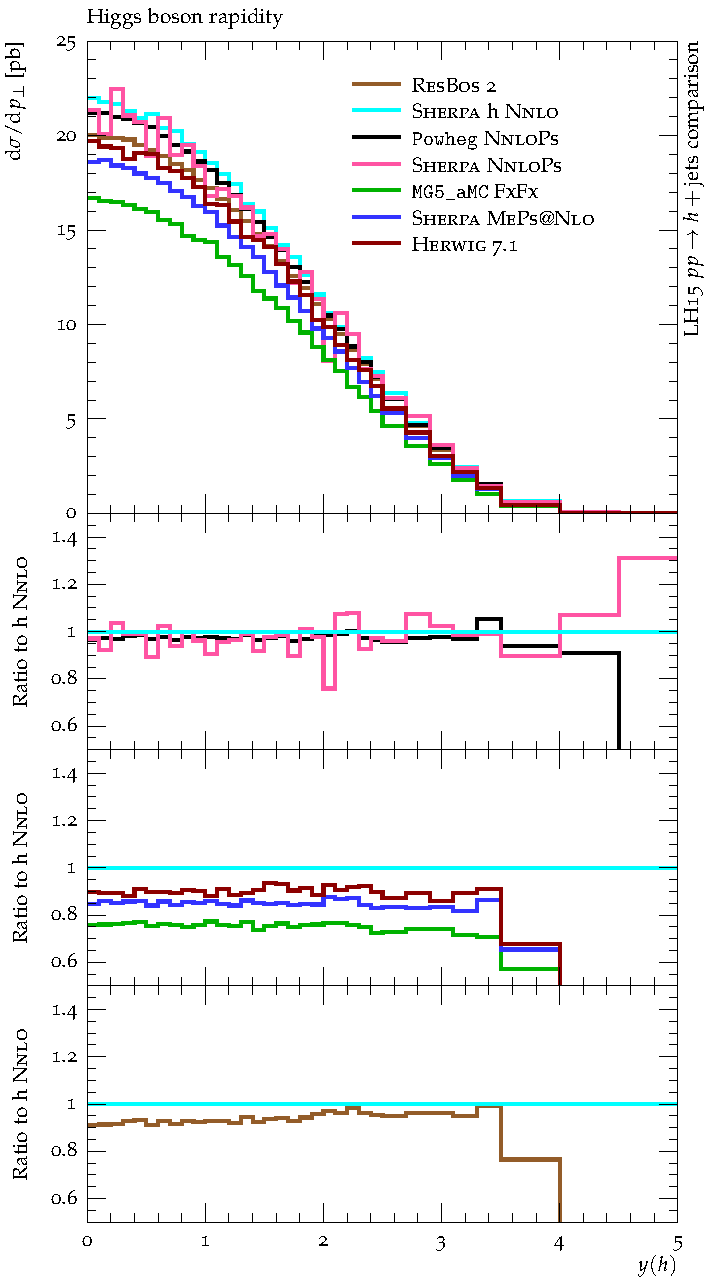
\includegraphics[width=0.47\textwidth]{figures/hjetscomp_u_H_y.pdf}
  \hfill
  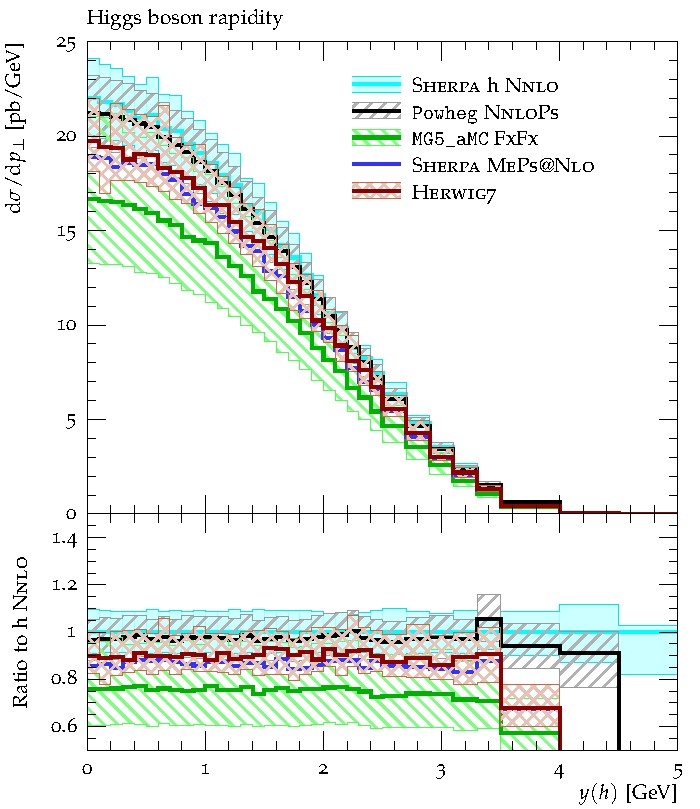
\includegraphics[width=0.47\textwidth]{figures/hjetscomp_H_y.pdf}
  \caption{\label{fig:higgscomp:results:inclobs:hy}%
    The inclusive Higgs boson rapidity without (left) and with (right)
    uncertainties. To enhance visibility, the NNLOPS and MEPS@NLO
    predictions are grouped together and shown wrt.~the same reference
    curve in the upper and lower ratio plots, respectively. The
    reference prediction is taken from the NNLO accurate description
    of inclusive $h$ production.}
\end{figure}

\Todo{I am confused here. It would seem to be natural to compare to
HNNLO for this variable, but the reference seems to be Sherpa h
NNLO. $\to$ Sherpa h NNLO is the same as HNNLO, shall we just call it
h NNLO instead and explain in text?}

We start by showing the inclusive Higgs boson rapidity distribution in
Figure~\ref{fig:higgscomp:results:inclobs:hy}. While the absolute
predictions are given in the top panel, the plots in the bottom panel
depict the respective ratios to the NNLO prediction. For better
visibility, we have divided the predictions into two groups based on
their simulation type and/or claimed accuracy. The upper ratio plot
contains the NNLO predictions while the lower one shows those obtained
from different strategies to merge matrix elements plus parton showers
at NLO. Overall, we find very good agreement in the description of the
shape of the $y(h)$ distribution. The main source of deviations stems
from the different normalizations given at NNLO or NLO and the
different (core) scale choices. As expected, the Sherpa NNLOPS and
Powheg NNLOPS results agree well with the pure NNLO prediction, while
MG5, Sherpa and Herwig7 have slightly lower (NLO) normalizations.
Here, the MG5 choice of a scale that reduces to $m_h$, rather than
$m_h/2$, is clearly noticeable. The upper edge of the MG5 uncertainty
band (equal to a scale that reduces to $m_h/2$) agrees with the
central value of the other NLO ME+PS predictions. There are no major
differences in the size of the uncertainty envelopes, although to some
extent, the NNLO scale uncertainty bands are smaller than those at NLO.
Note that the NLO-based predictions fall off more rapidly at higher
$y$ than do the NNLO-based predictions. This is expected because of
the influence of additional $ln(1-x)$ corrections present in the
determination of NNLO PDFs. Similar effects can be observed in going
from LO to NLO.

\Todo{Do we say in the technicalities section how error bands are
  obtained? Or do we rather say it at the appropriate places when
  describing the plots?}

\begin{figure}[t!]
  \centering
  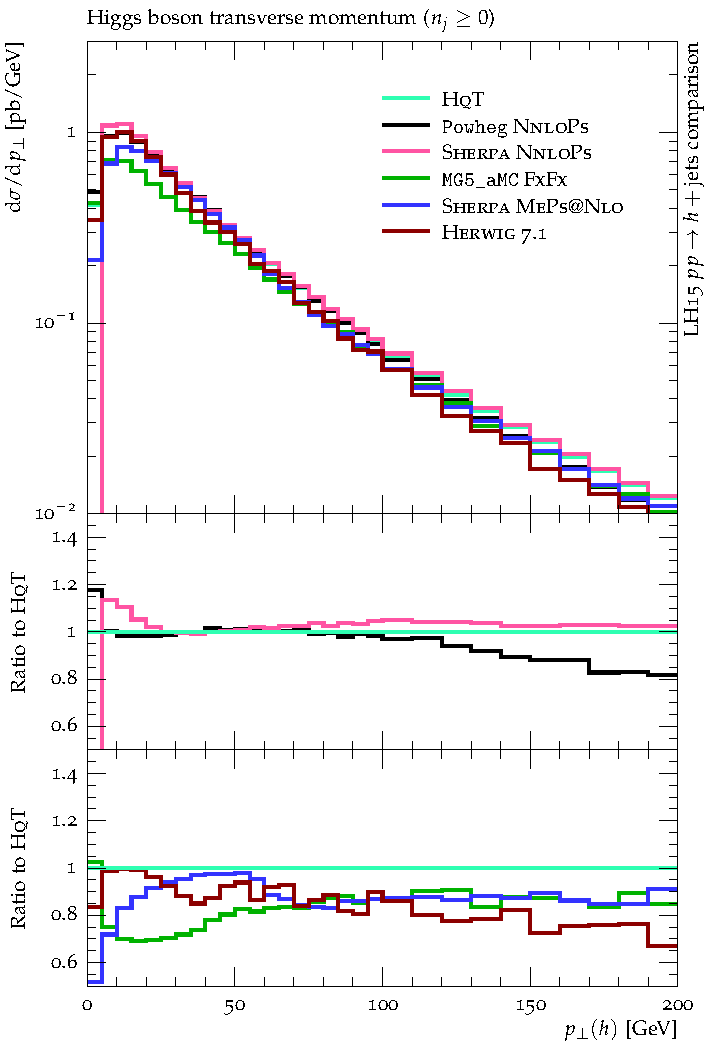
\includegraphics[width=0.47\textwidth]{figures/hjetscomp_u_H_pT_incl.pdf}
  \hfill
  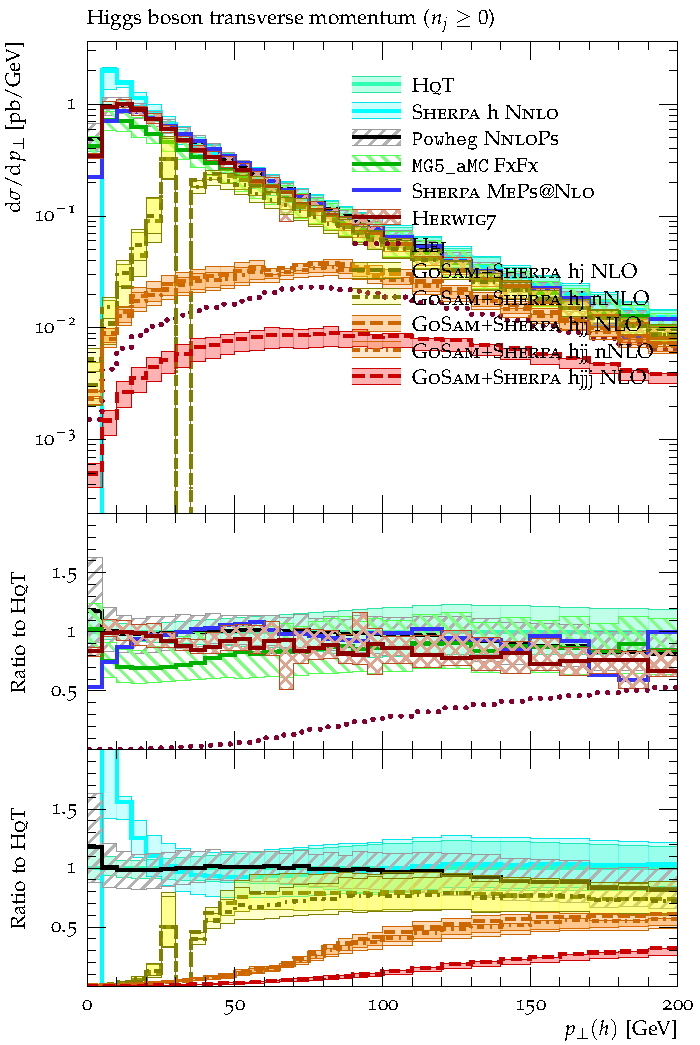
\includegraphics[width=0.47\textwidth]{figures/hjetscomp_H_pT_incl.pdf}
  \caption{\label{fig:higgscomp:results:inclobs:hpt}%
    The Higgs boson transverse momentum in the inclusive event selection
    without (left) and with (right) uncertainties. For the ratios in
    the bottom panel, the same grouping strategy has been used as in
    Figure~\ref{fig:higgscomp:results:inclobs:hy}, while the reference
    prediction has been changed from that of pure NNLO to the one
    given by HqT.}
\end{figure}

In Figure~\ref{fig:higgscomp:results:inclobs:hpt}, the inclusive Higgs
boson transverse momentum distribution is shown, with the ratio to HqT
(Powheg NNLOPS) in the bottom panel.  In general, good agreement with
HqT is observed, with some deviations evident at very low $p_T$.  The
fixed order predictions are neither stable (nor reliable) at low
$p_T$, as expected since this is a strong Sudakov region. The Powheg
prediction seems to fall off more rapidly at high $p_T$. Note the MG5
central scale choice becomes less significant as the Higgs boson
transverse momentum increases.

\begin{figure}[t!]
  \centering
  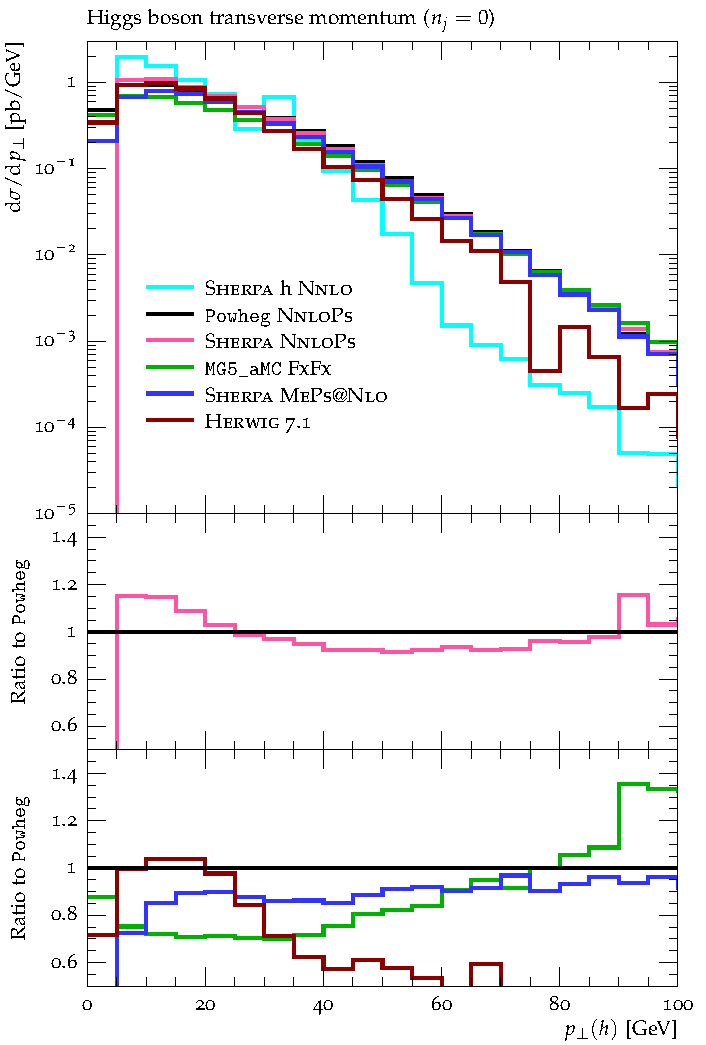
\includegraphics[width=0.47\textwidth]{figures/hjetscomp_u_H_pT_excl.pdf}
  \hfill
  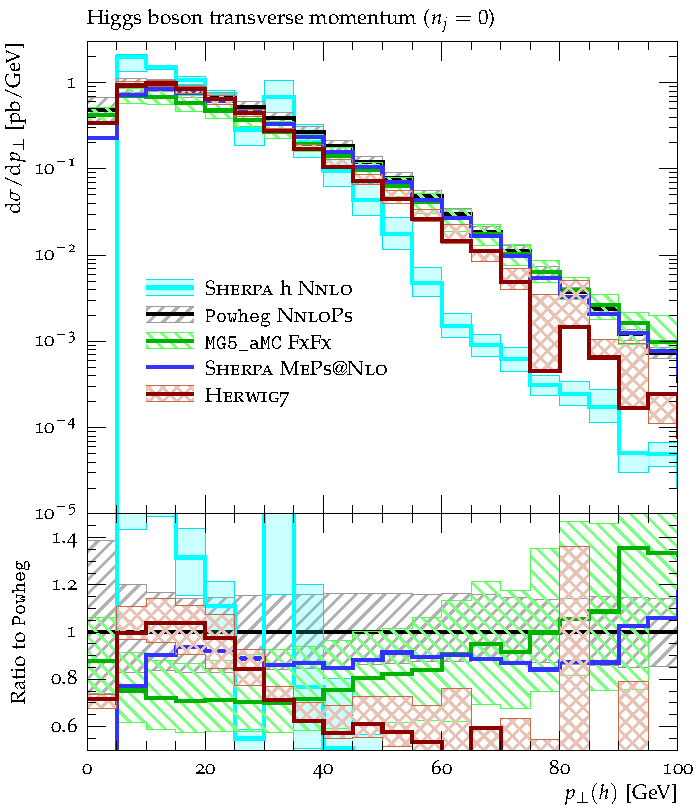
\includegraphics[width=0.47\textwidth]{figures/hjetscomp_H_pT_excl.pdf}
  \caption{
    The Higgs boson transverse momentum in the exclusive event
    selection (i.e.~in the absence of any jet) without (left) and with
    (right) uncertainties.
    \label{fig:higgscomp:results:exclobs:hpt}
  }
\end{figure}

The exclusive Higgs boson transverse momentum distribution (no jets
above 30 GeV/c) is shown in
Figure~\ref{fig:higgscomp:results:exclobs:hpt}. Here, the deviations
among predictions above 30 GeV/c become more sizable. This is a
stringent test of ME+PS predictions, as the high transverse momentum
is produced by a combination of soft jets (below 30 GeV/c) and soft
gluon radiation, and the deviation of the predictions is probably a
good reflection of the true uncertainty.

\begin{figure}[t!]
  \centering
  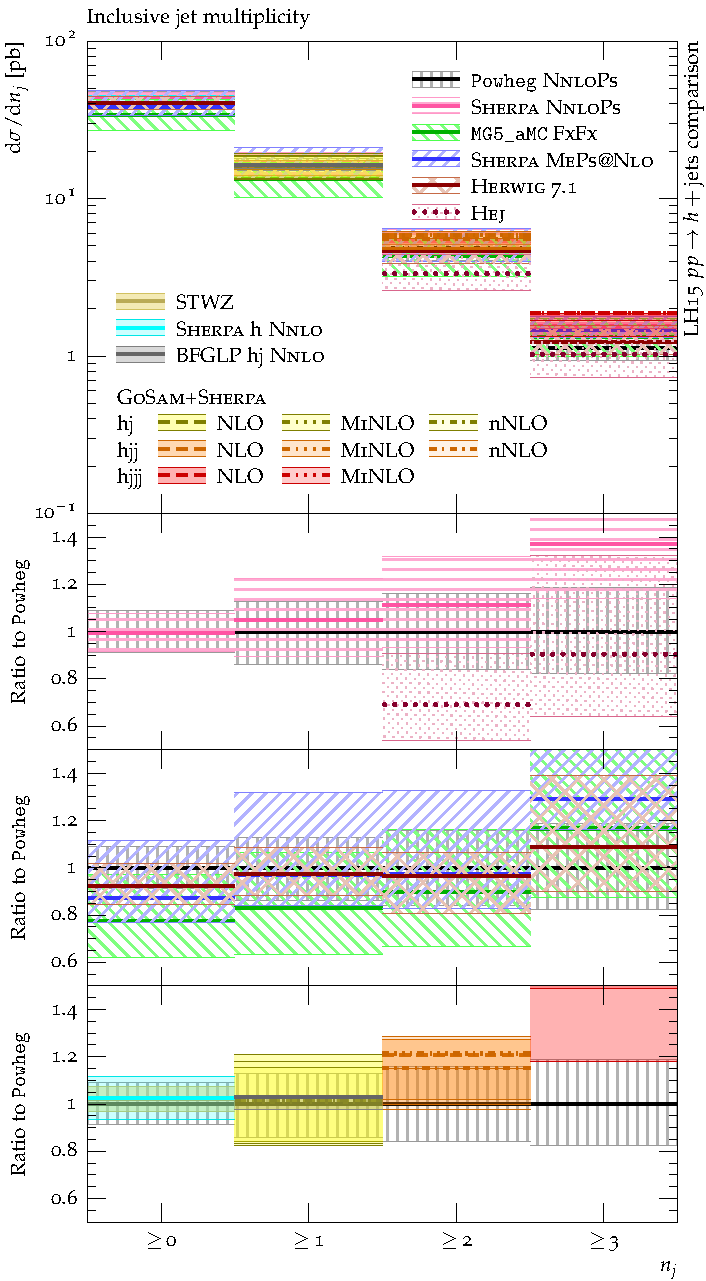
\includegraphics[width=0.47\textwidth]{figures/hjetscomp_NJet_incl_30.pdf}
  \hfill
  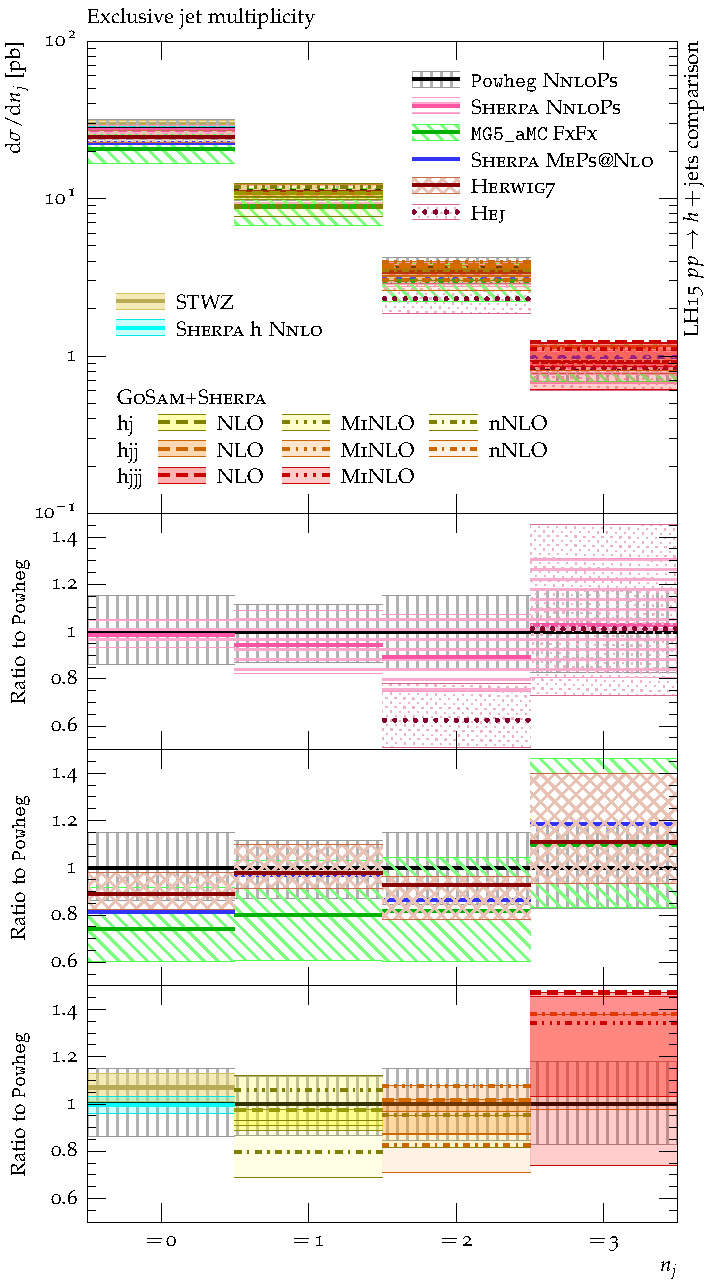
\includegraphics[width=0.47\textwidth]{figures/hjetscomp_NJet_excl_30.pdf}
  \caption{
    The inclusive (left) and exclusive (right) jet multiplicities.
    \label{fig:higgscomp:results:inclobs:njets}
  }
\end{figure}

The inclusive and exclusive jet multiplicity distributions are shown
in Figure~\ref{fig:higgscomp:results:inclobs:njets}. Fixed order
predictions at NLO are shown for all jet multiplicities, at NNLO for
the 1 jet bin, and at approximate NNLO (LoopSim) for the 1 and 2 jet
bins. Unlike the inclusive Higgs production case, the NNLO corrections
for inclusive 1 jet production are small (slightly negative for this
central scale choice). There is a notable decrease in the scale
uncertainty. In general, good agreement for the jet multiplicity
predictions is observed, except in the 3 jet bin (both inclusive and
exclusive), where the gosam prediction shows the NLO corrections
absent in the other predictions.



\clearpage
\subsection{One-jet observables}
\label{sec:hjetscomp:results:1jobs}

\begin{figure}[t!]
  \centering
  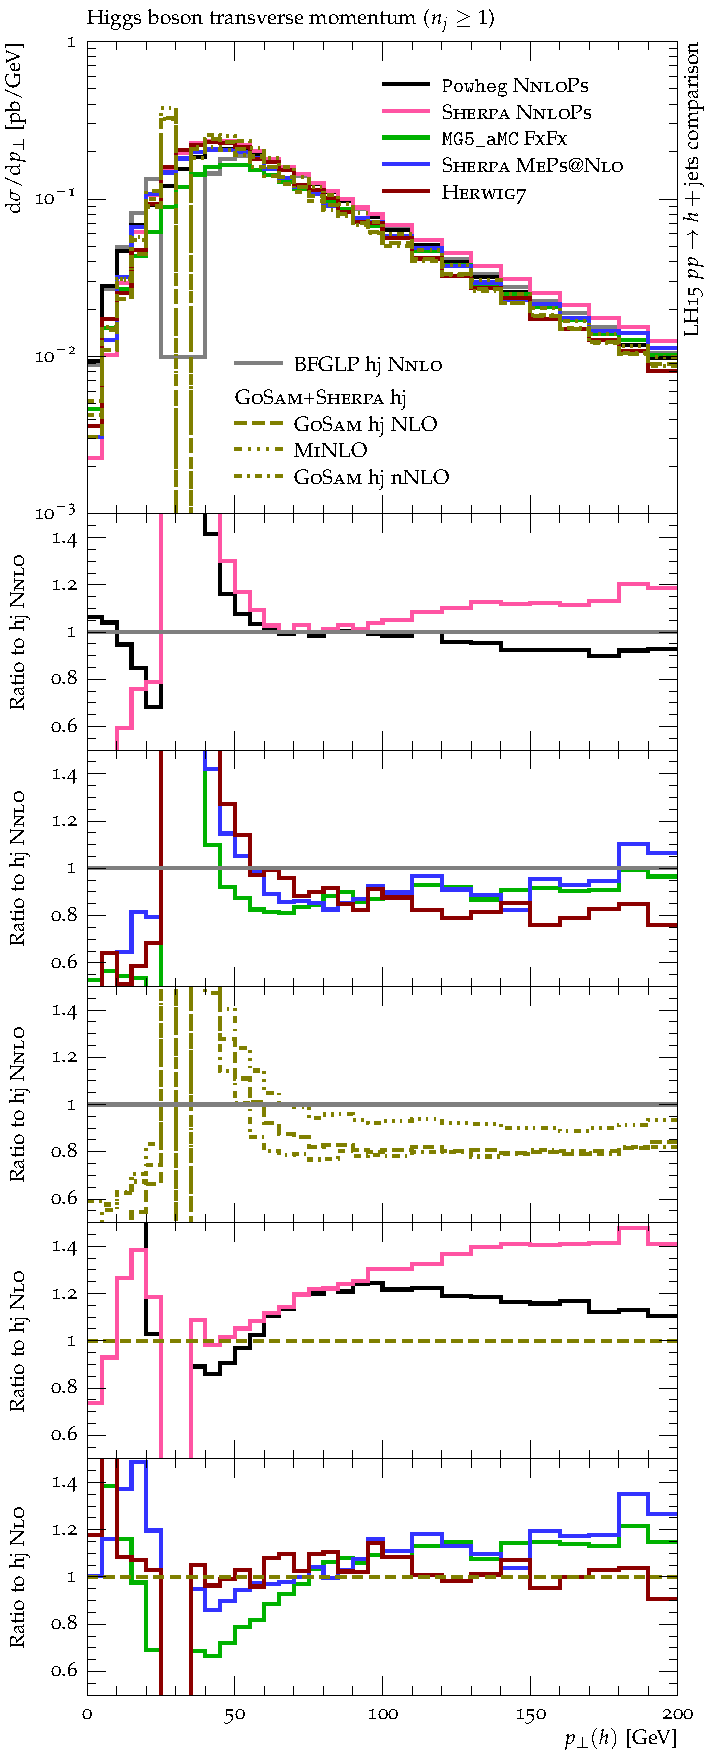
\includegraphics[width=0.47\textwidth]{figures/hjetscomp_u_H_j_pT_incl.pdf}
  \hfill
  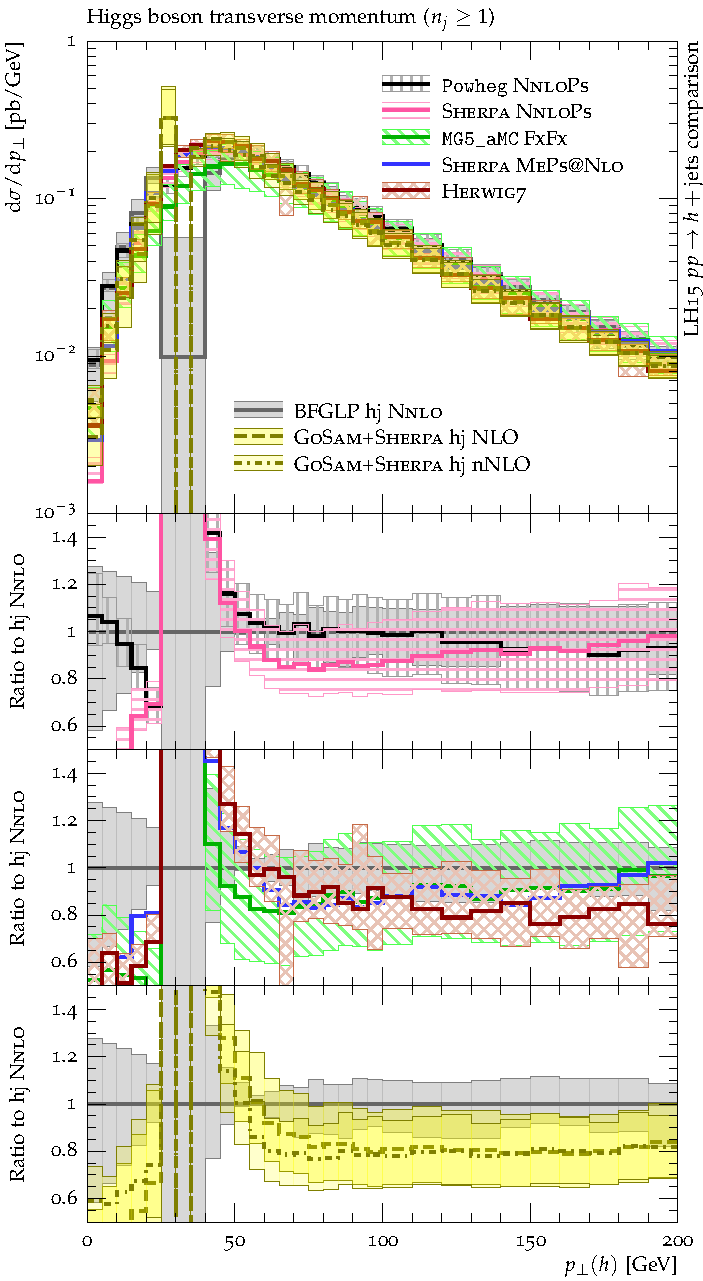
\includegraphics[width=0.47\textwidth]{figures/hjetscomp_H_j_pT_incl.pdf}
  \caption{
    The Higgs boson transverse momentum in the presence of at least
    one jet without (left) and with (right) uncertainties.
    \label{fig:higgscomp:results:1obs:hpt}
  }
\end{figure}

\begin{figure}[t!]
  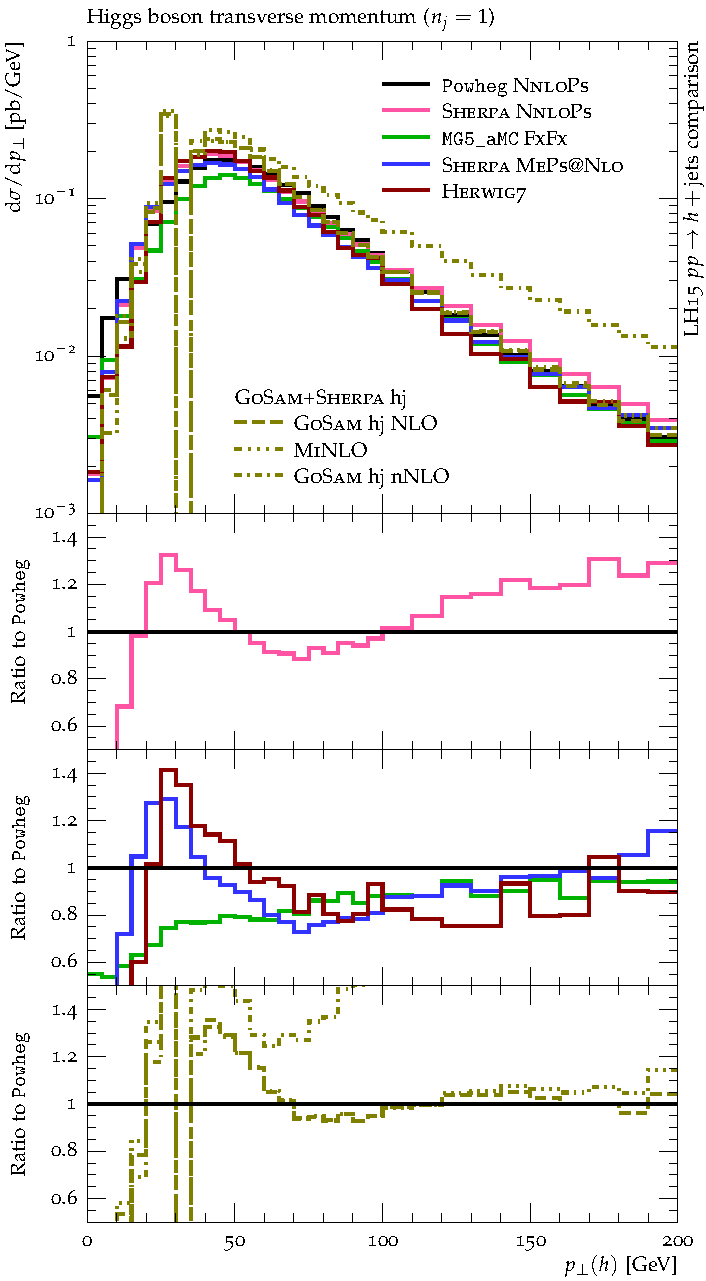
\includegraphics[width=0.47\textwidth]{figures/hjetscomp_u_H_j_pT_excl.pdf}
  \hfill
  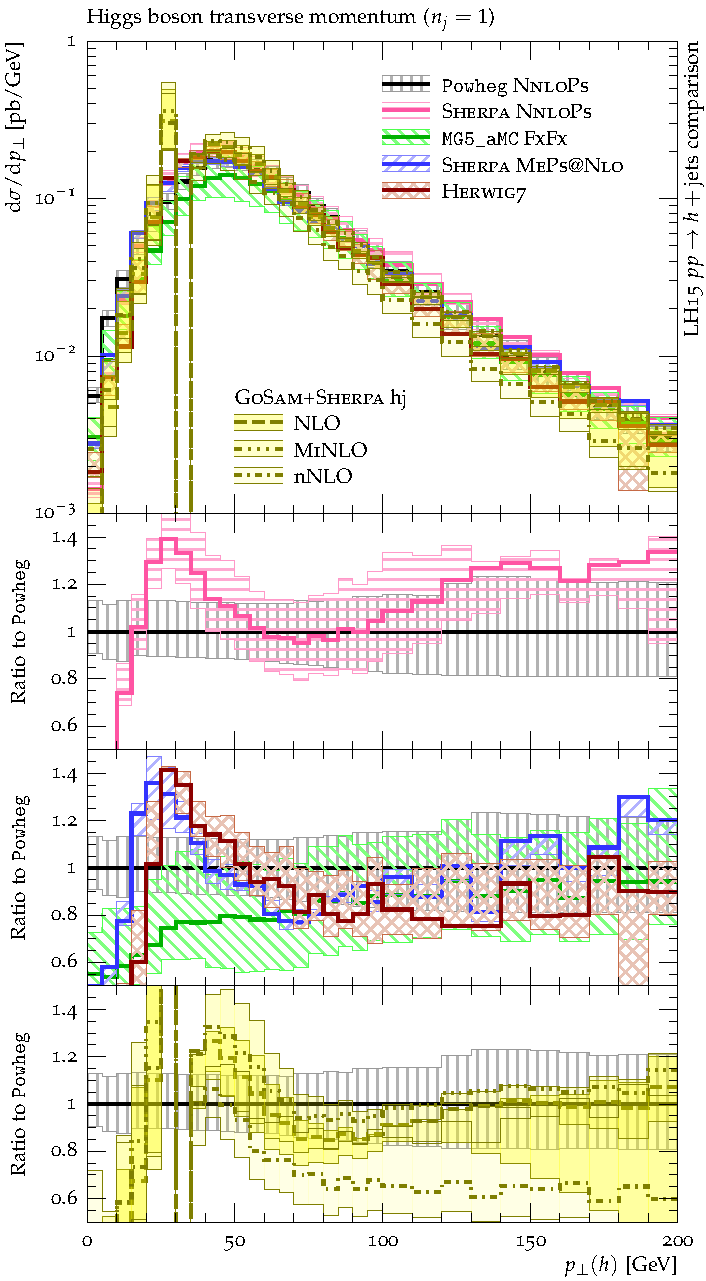
\includegraphics[width=0.47\textwidth]{figures/hjetscomp_H_j_pT_excl.pdf}
  \caption{
    The Higgs boson transverse momentum in the presence of at exactly 
    one jet without (left) and with (right) uncertainties.
    \label{fig:higgscomp:results:1obs:hpt_excl}
  }
\end{figure}

The Higgs boson transverse momentum distribution with the presence of
at least one jet is shown in
Figure~\ref{fig:higgscomp:results:1obs:hpt}. These are variables for
which large Sudakov effects are expected at low $p_T$ and indeed the
fixed order predictions are somewhat unstable for transverse momenta
less than 50 GeV/c. There are also shape differences between the ME+PS
predictions at low $p_T$. For high $p_T$, the predictions are in
better overall agreement with each other and with the NNLO
prediction. The upper edge of the MG5 error band (corresponding to the
nominal central scaler) is noticeable higher than the other
predictions.

The Higgs boson transverse momentum distribution with the presence of
exactly one jet is shown in
Figure~\ref{fig:higgscomp:results:1obs:hpt_excl}. In this case, the
differences with respect to Powheg become larger for the full
tranverse momentum range.

\Todo{concerning the two previous paragraphs $\to$ physics?}

\begin{figure}[t!]
  \centering
  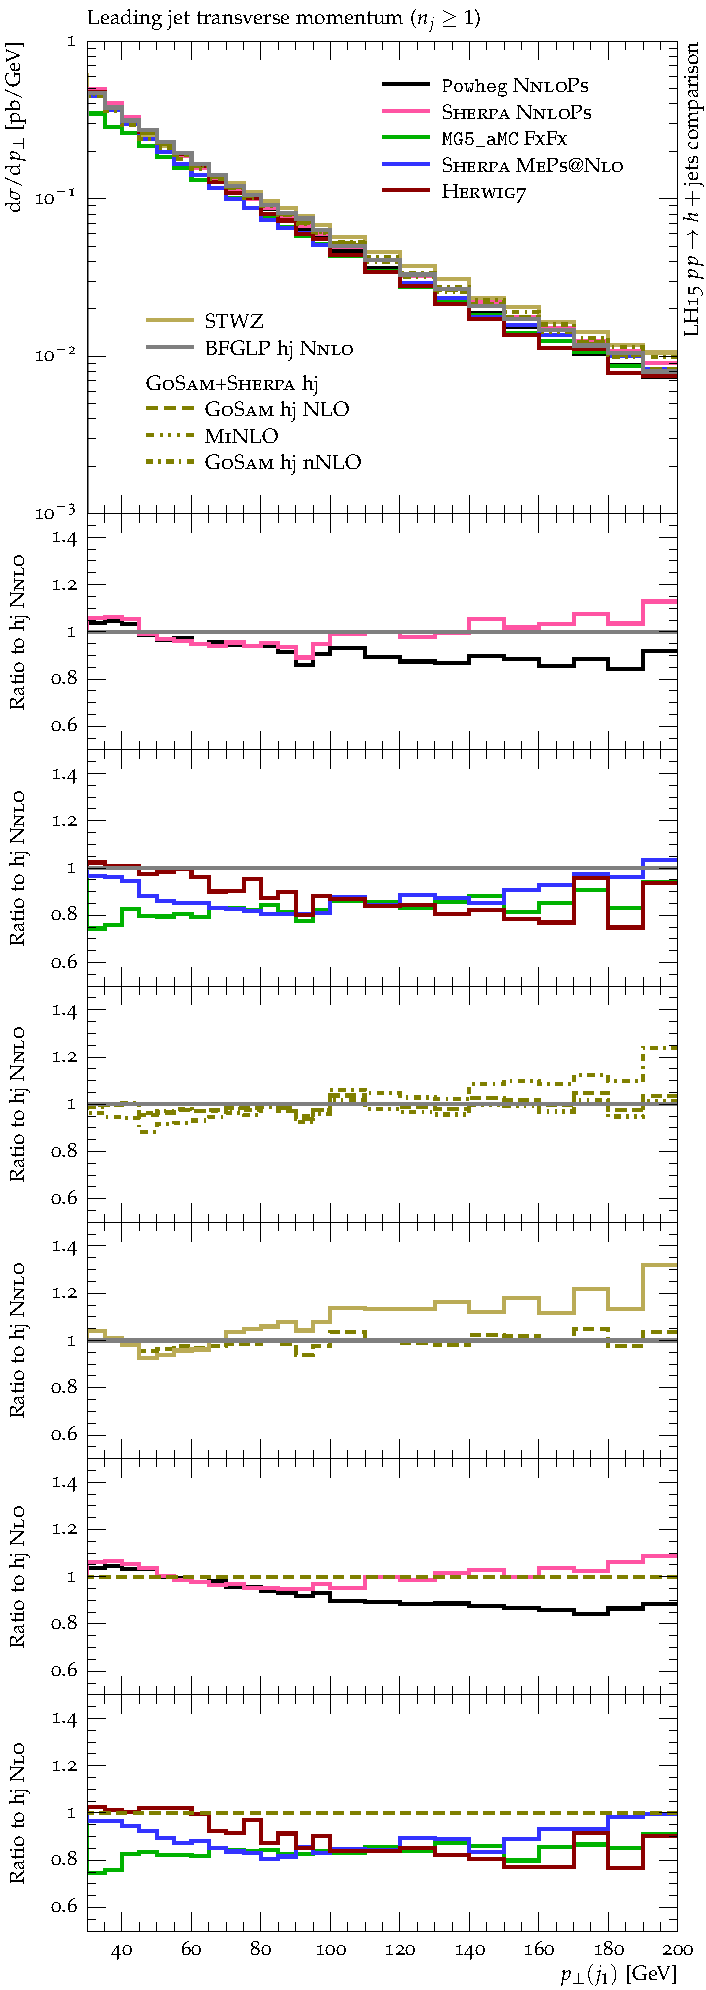
\includegraphics[width=0.47\textwidth]{figures/hjetscomp_u_jet1_pT_incl.pdf}
  \hfill
  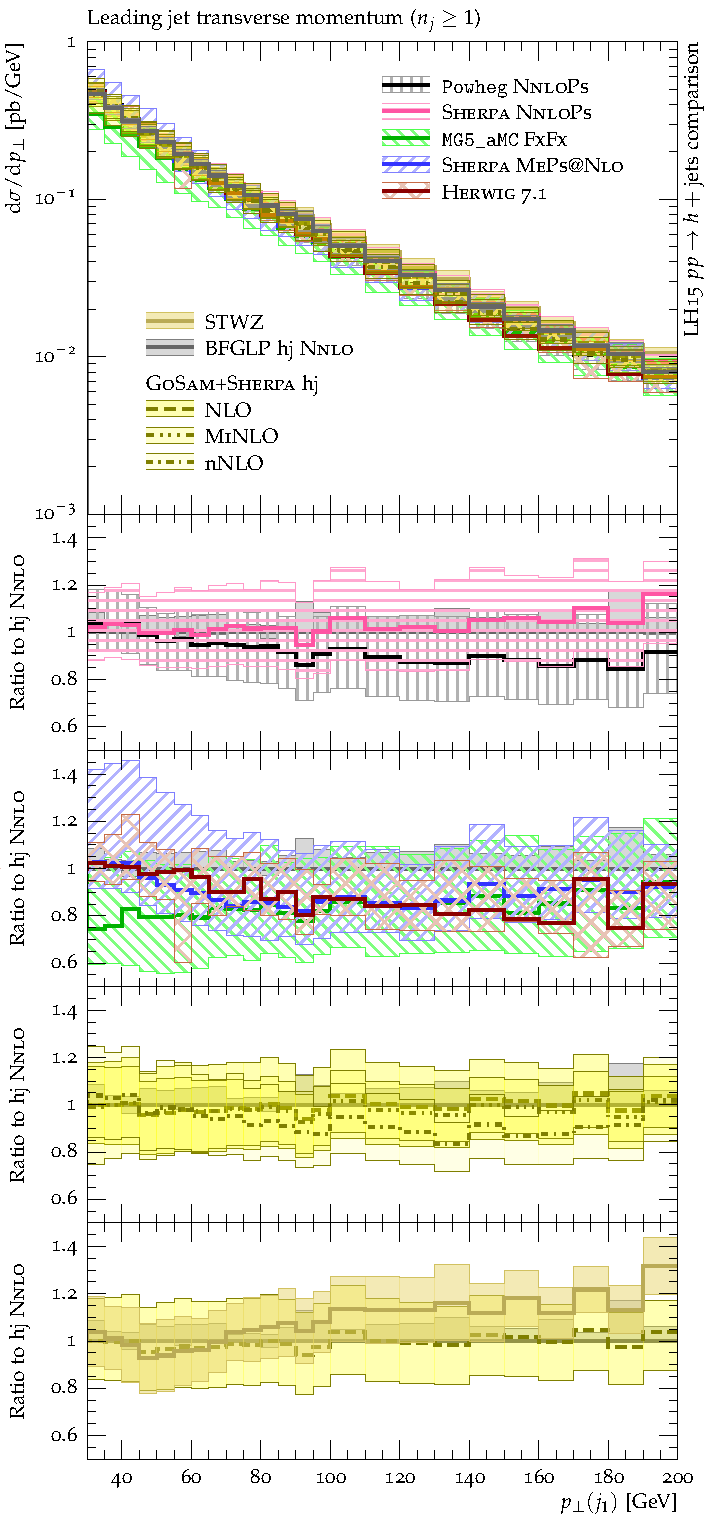
\includegraphics[width=0.47\textwidth]{figures/hjetscomp_jet1_pT_incl.pdf}
  \caption{
    The inclusive leading jet transverse momentum distribution for
    $H+\ge1$ jet production without (left) and with (right) uncertainties.
    \label{fig:higgscomp:results:1obs:j1pt}
  }
\end{figure}

The lead jet transverse momentum distribution for $H+\ge1$ jet is
shown in Figure~\ref{fig:higgscomp:results:1obs:j1pt}.

In the middle panel, the ratio of the ME+PS predictions to Powheg is
shown. Sherpa and Herwig7 have somewhat of a slope difference with
respect to Powheg in the jet transverse momentum range of 30-100
GeV/c, while MG5 (with its different central scale choice) is in
agreement with Powheg over the kinematic range shown.  In the bottom
panel, Powheg and gosam NLO and nNLO (using LoopSim) are compared (in
ratio) to the NNLO prediction for the lead jet transverse
momentum. Gosam NLO is above the NNLO prediction in the lead jet
transverse momentum range for 30-50 GeV/c, but in agreement above that
range. Powheg, with its central scale choice, is approximately 30\%
higher than the NNLO prediction for $p_T^{jet}=30$ GeV/c, and in
better agreement for $p_T^{jet}=100$ GeV/c. Thus, the central Powheg
prediction is in somewhat larger disagreement with the NNLO prediction
than with the NLO prediction in the low $p_T$ range. The nNLO
(LoopSim) prediction starts above the NNLO prediction, but then is
about 10-15\% lower for higher $p_T^{jet}$ values. The gosam MINLO
results are about 20\% higher than the nominal gosam NLO results, so
closer to Powheg at low $p_T$, but higher than Powheg at high $p_T$.

Note that for this observable, we do not expect large Sudakov effects
(i.e. shifts due to parton showering/resummation). The impact of jet
veto logarithms (due to the restriction that all jets be greater than
30 GeV/c) has been examined and found to be reasonably small at NLO
and NNLO~\cite{monni}.

\Todo{provide numbers from Monni?}
\Todo{Do we have any?}

\begin{figure}[t!]
  \centering
  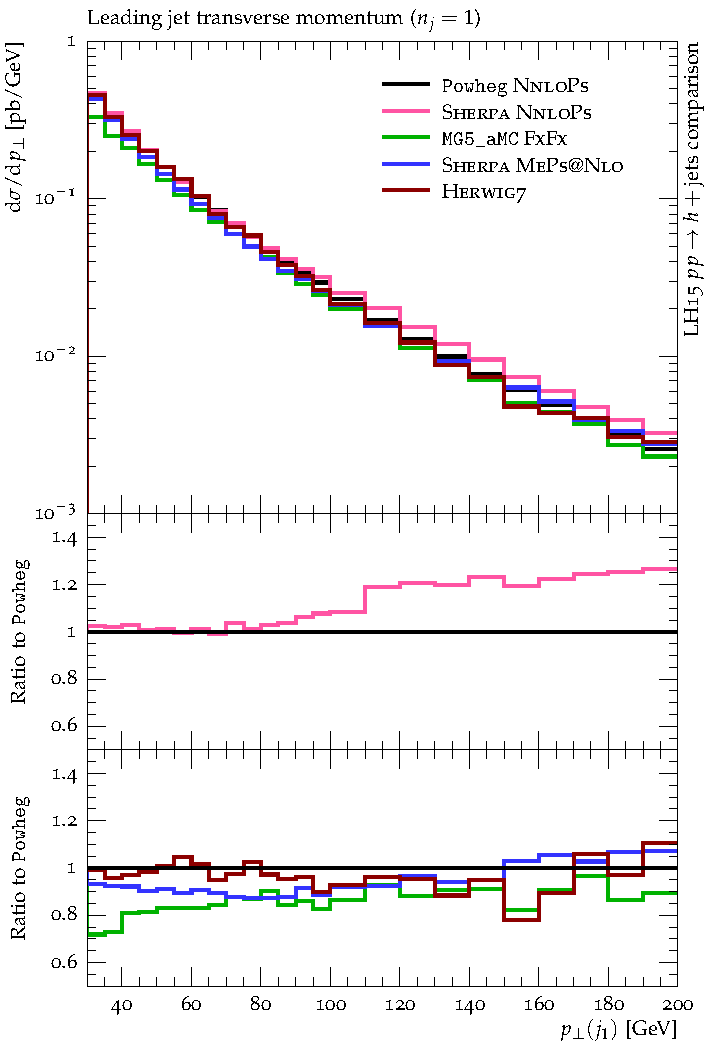
\includegraphics[width=0.47\textwidth]{figures/hjetscomp_u_jet1_pT_excl.pdf}
  \hfill
  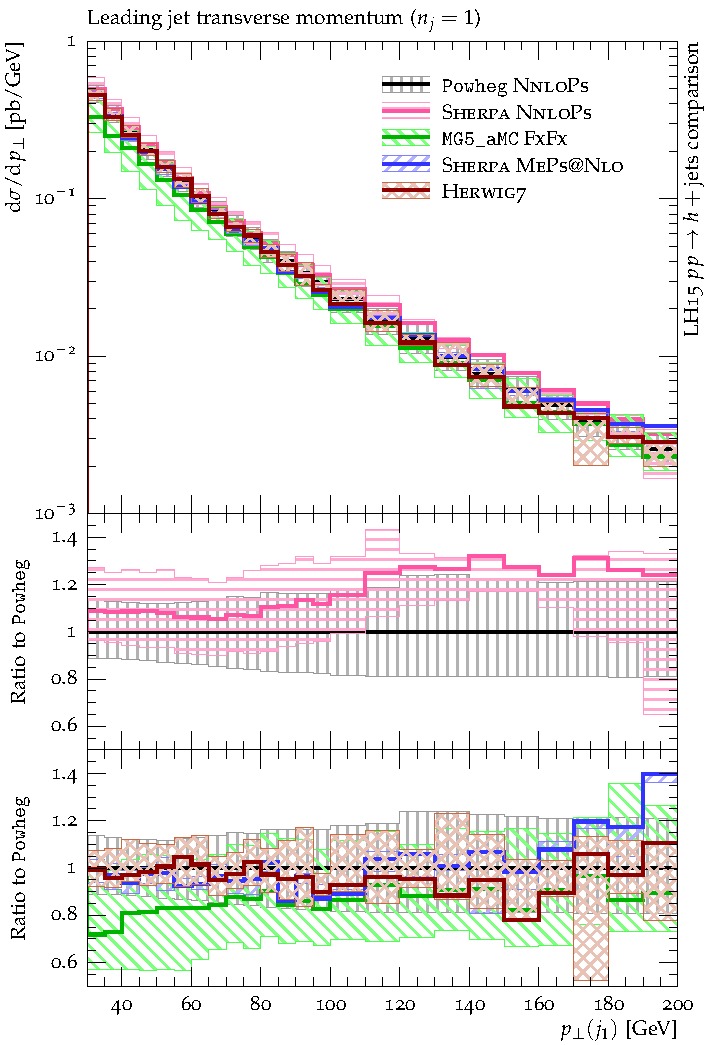
\includegraphics[width=0.47\textwidth]{figures/hjetscomp_jet1_pT_excl.pdf}
  \caption{
    The exclusive leading jet transverse momentum distribution for
    $H+\ge1$ jet production without (left) and with (right) uncertainties.
    \label{fig:higgscomp:results:1obs:j1pt_excl}
  }
\end{figure}

The exclusive lead jet transverse momentum distribution is shown in
Figure~\ref{fig:higgscomp:results:1obs:j1pt_excl}. All predictions are
in reasonably good agreement with Powheg. The MG5 prediction is lower
than Powheg for basically the entire transverse momentum range, again
because of the central scale choice. Note that this is a variable in a
strong Sudakov region, and the scale uncertainties shown do not
reflect the true uncertainty.

\begin{figure}[t!]
  \centering
  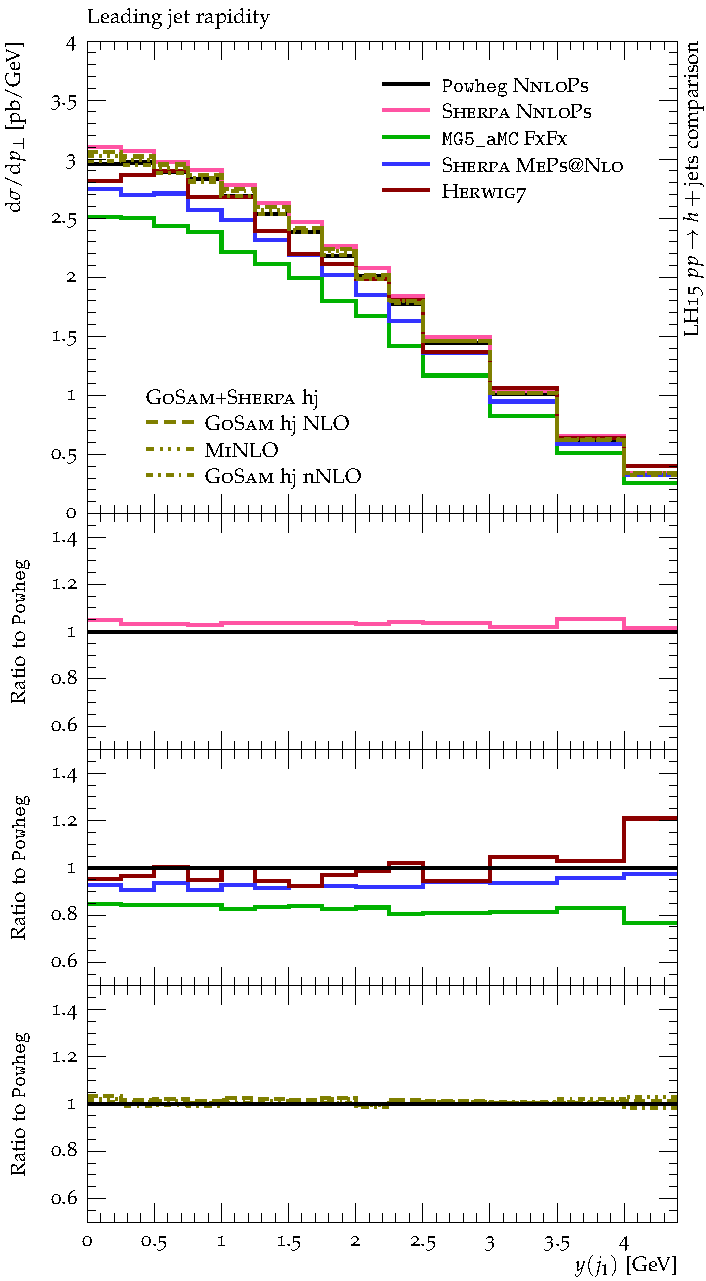
\includegraphics[width=0.47\textwidth]{figures/hjetscomp_u_jet1_y.pdf}
  \hfill
  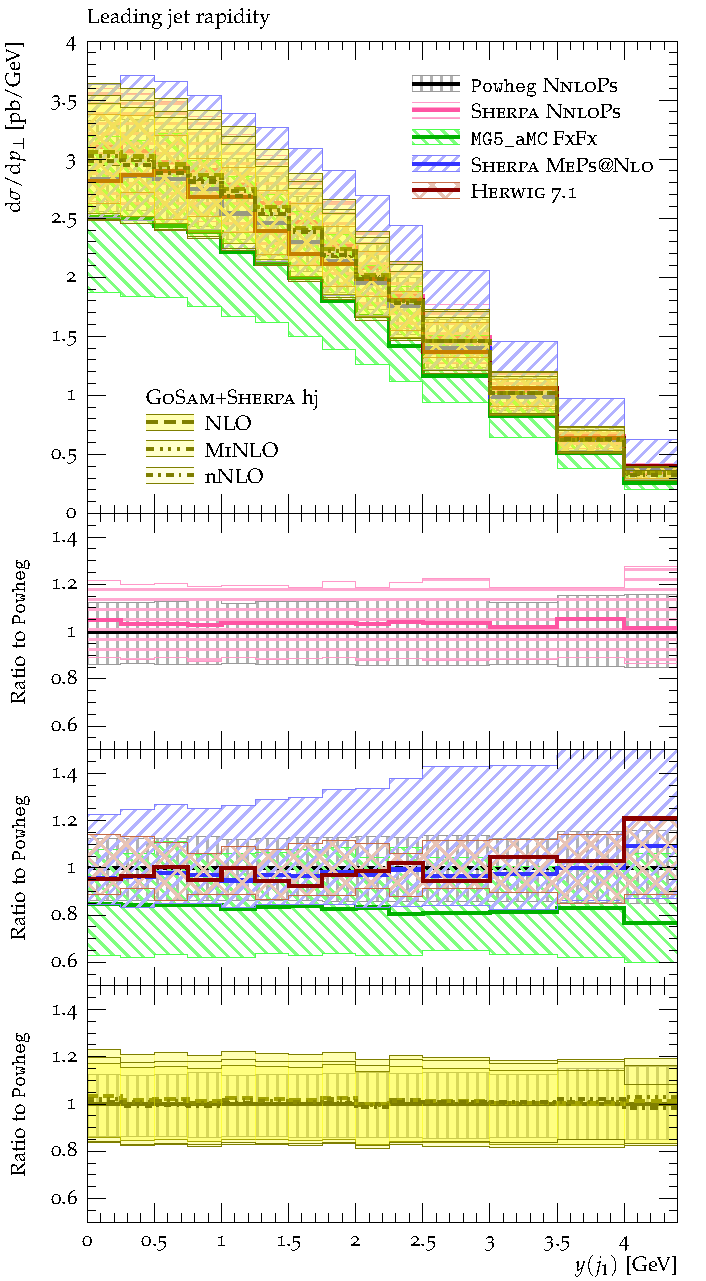
\includegraphics[width=0.47\textwidth]{figures/hjetscomp_jet1_y.pdf}
  \caption{
    The rapidity distribution for the leading jet in $H+\ge1$ jet production
    without (left) and with (right) uncertainties. 
    \label{fig:higgscomp:results:1obs:j1y}
  }
\end{figure}

The rapidity distribution for the lead jet is shown in
Figure~\ref{fig:higgscomp:results:1obs:j1y}.

\begin{figure}[t!]
  \centering
  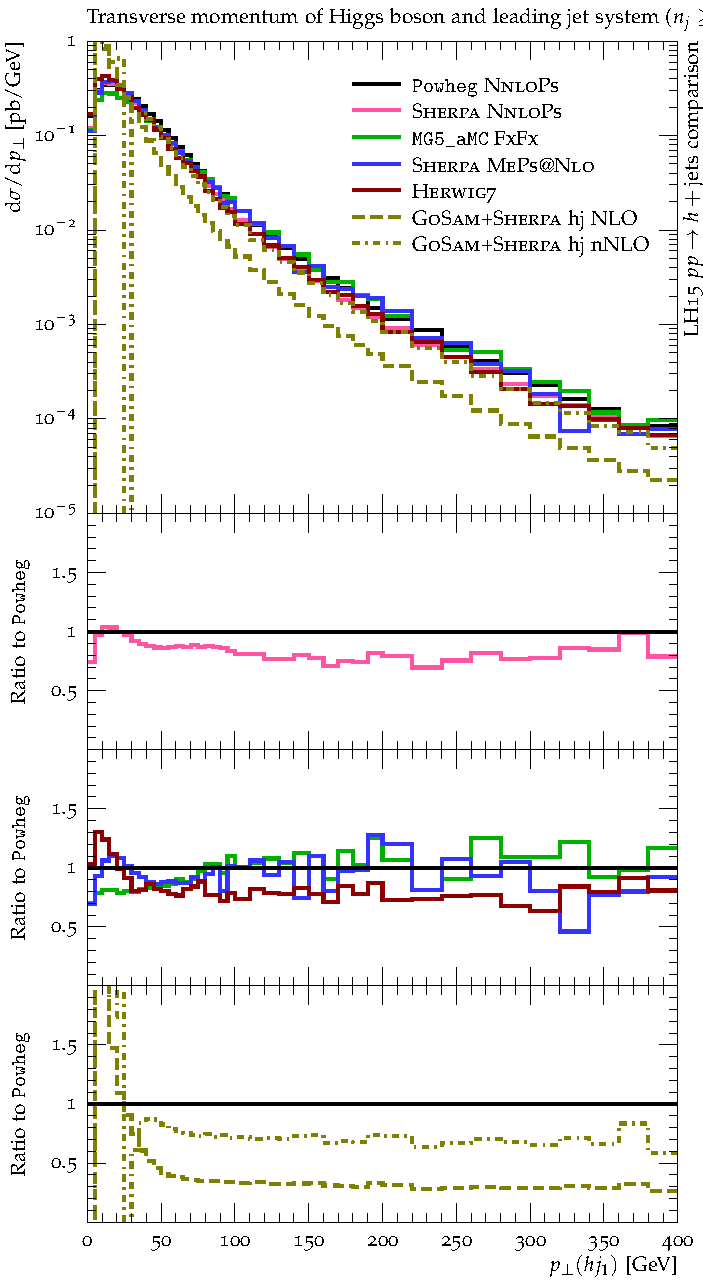
\includegraphics[width=0.47\textwidth]{figures/hjetscomp_u_Hj_pT_incl.pdf}
  \hfill
  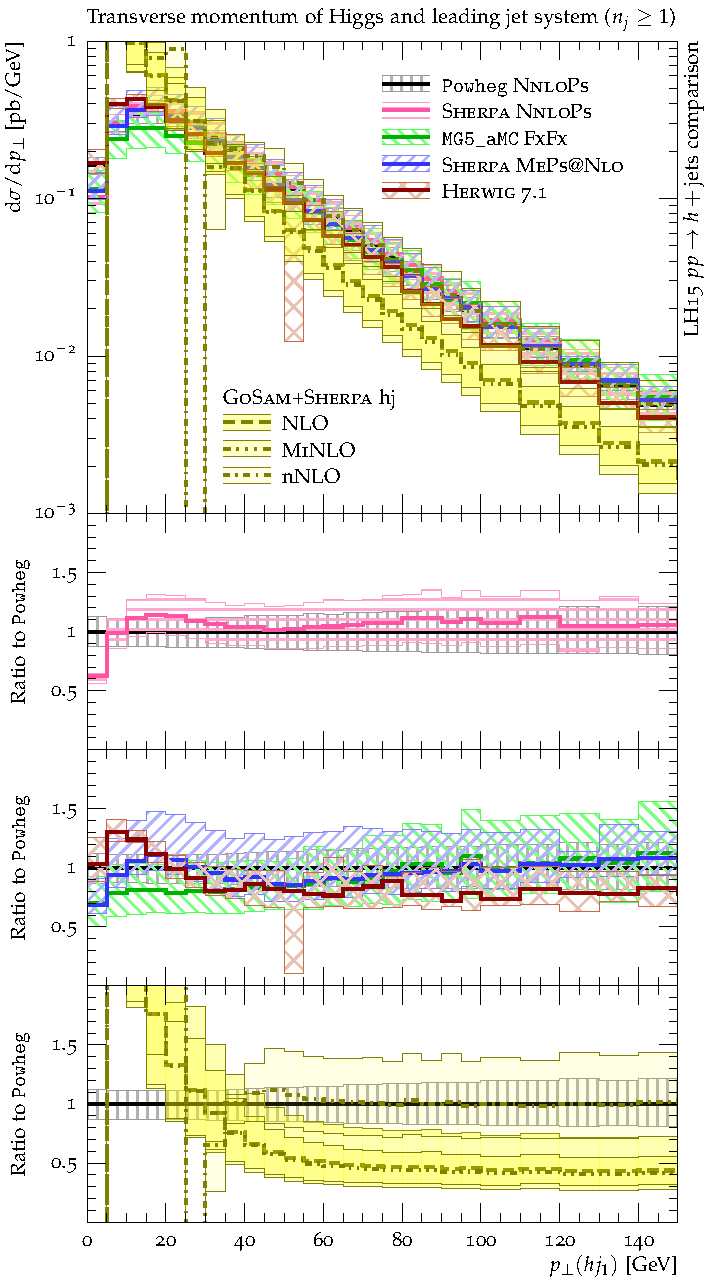
\includegraphics[width=0.47\textwidth]{figures/hjetscomp_Hj_pT_incl.pdf}
  \caption{
    The transverse momentum of the Higgs-boson-leading-jet system in the 
    presence of at least one jet without (left) and with (right) uncertainties.
    \label{fig:higgscomp:results:1obs:hj_pt}
  }
\end{figure}

\begin{figure}[t!]
  \centering
  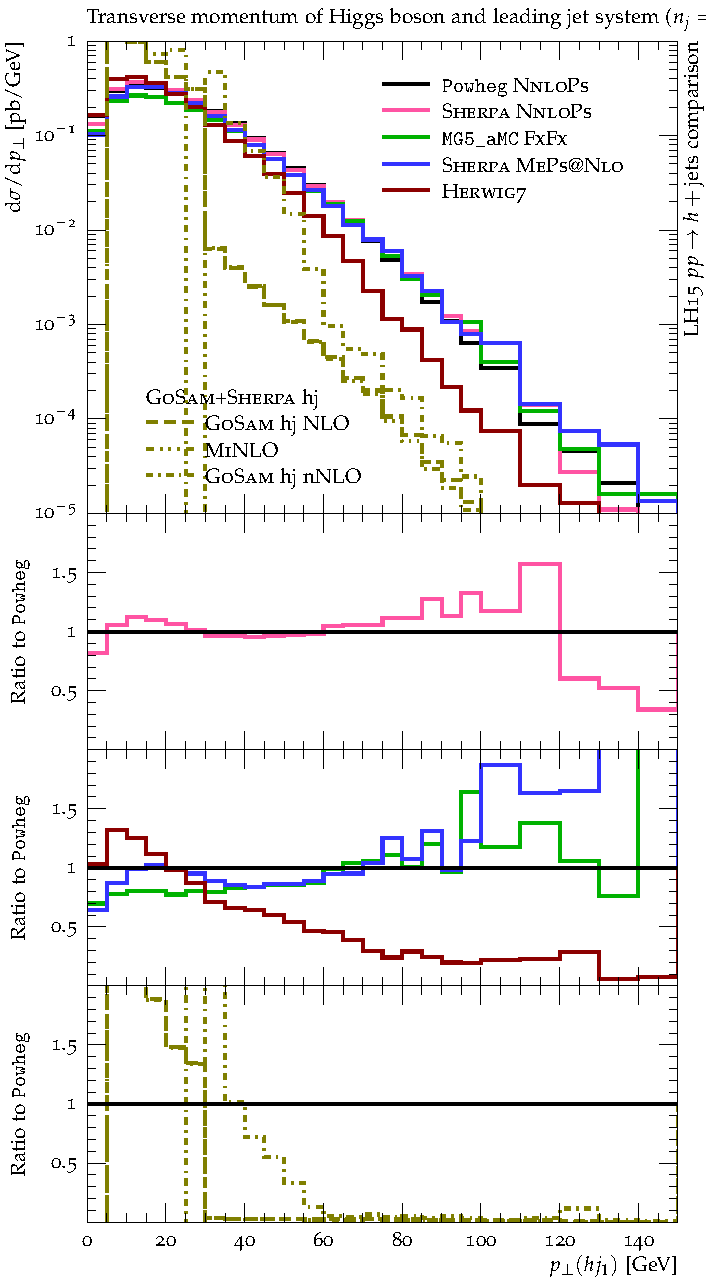
\includegraphics[width=0.47\textwidth]{figures/hjetscomp_u_Hj_pT_excl.pdf}
  \hfill
  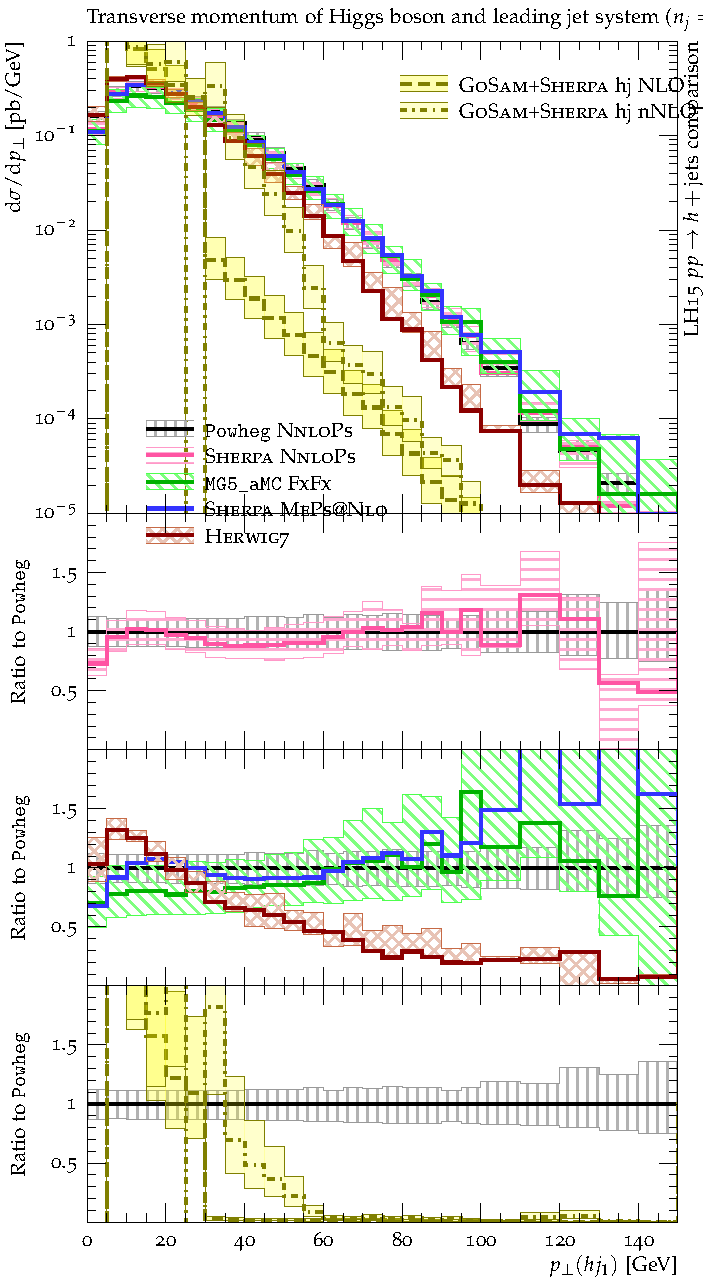
\includegraphics[width=0.47\textwidth]{figures/hjetscomp_Hj_pT_excl.pdf}
  \caption{
    The transverse momentum of the Higgs-boson-leading-jet system in the 
    presence of exactly one jet without (left) and with (right) uncertainties.
    \label{fig:higgscomp:results:1obs:hj_pt_excl}
  }
\end{figure}

Next we examine the transverse momentum of the Higgs boson + leading
jet system. The inclusive case ($\ge 1$ jet) is shown in the upper
part of Figure~\ref{fig:higgscomp:results:1obs:hj_pt}.  Again,
differences can be observed for the $\ge 1$ jet ME+PS predictions at
low $p_T$, while there is better agreement at higher $p_T$.

\Todo{but what is happening with MG5 at high pT}

The exclusive case (exactly jet) is shown in the lower part of
Figure~\ref{fig:higgscomp:results:1obs:hj_pt}.  There is a much
greater divergence of the predictions for exactly one jet, especially
at high $p_T$.  A highly exclusive distribution such as this serves as
a stress test for ME+PS prediction, similar to the case for the Higgs
$p_T$ distribution with no jets and it is no surprise that different
approaches can lead to different answers.



\clearpage
\subsection{Dijet observables}
\label{sec:hjetscomp:results:2jobs}

\begin{figure}[t!]
  \centering
  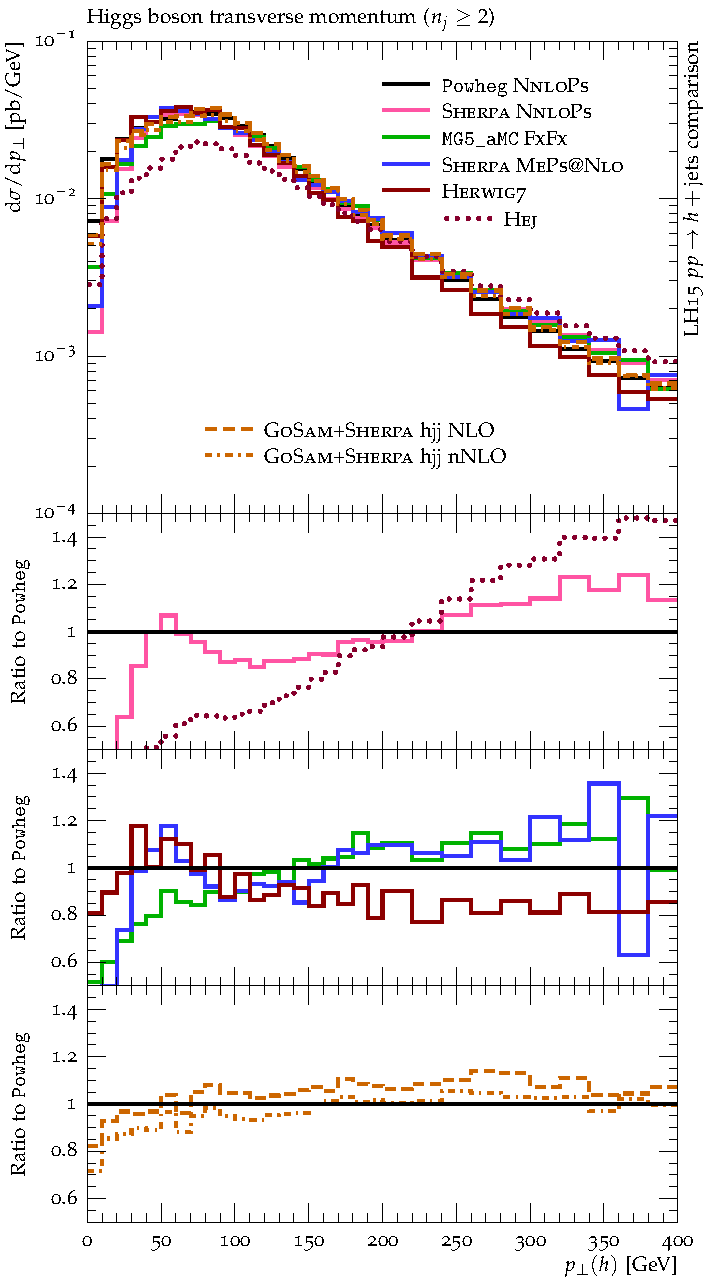
\includegraphics[width=0.47\textwidth]{figures/hjetscomp_u_H_jj_pT_incl.pdf}
  \hfill
  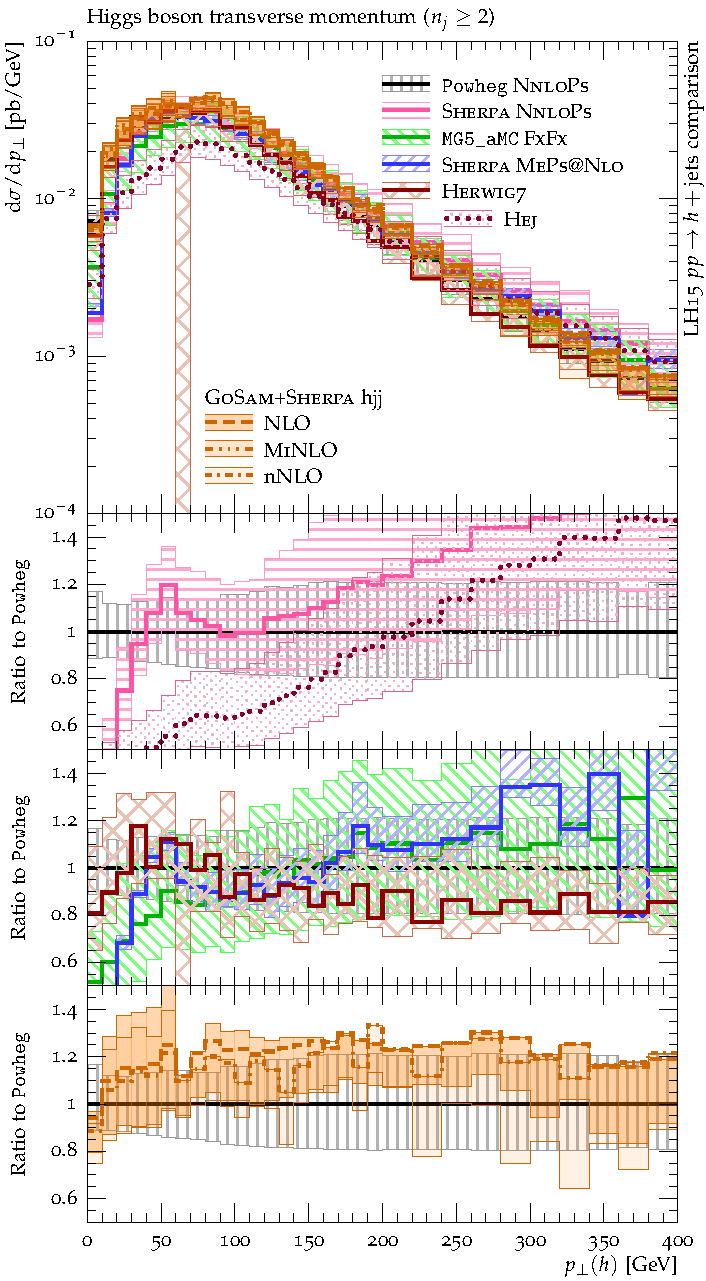
\includegraphics[width=0.47\textwidth]{figures/hjetscomp_H_jj_pT_incl.pdf}
  \caption{
    The transverse momentum of the Higgs boson in the presence
    of at least two jets without (left) and with (right) uncertainties.
    \label{fig:higgscomp:results:2obs:hpt_j2pt}
  }
\end{figure}

The Higgs boson $p_T$, in the presence of at least two jets, is shown
in Figure~\ref{fig:higgscomp:results:2obs:hpt_j2pt}. Here, varying
behavior is observed, with MG5 and Sherpa being substantially lower
than Powheg at low $p_T$ and somewhat higher at high $p_T$, while
Herwig7 is somewhat lower than Powheg at high $p_T$. The gosam
$H+\ge2$ jet prediction is lower than Powheg at low $p_T$ (as expected
for a Sudakov region),and roughly 10\% higher at high $p_T$ (closer to
the MG5/Sherpa predictions).

\begin{figure}[t!]
  \centering
  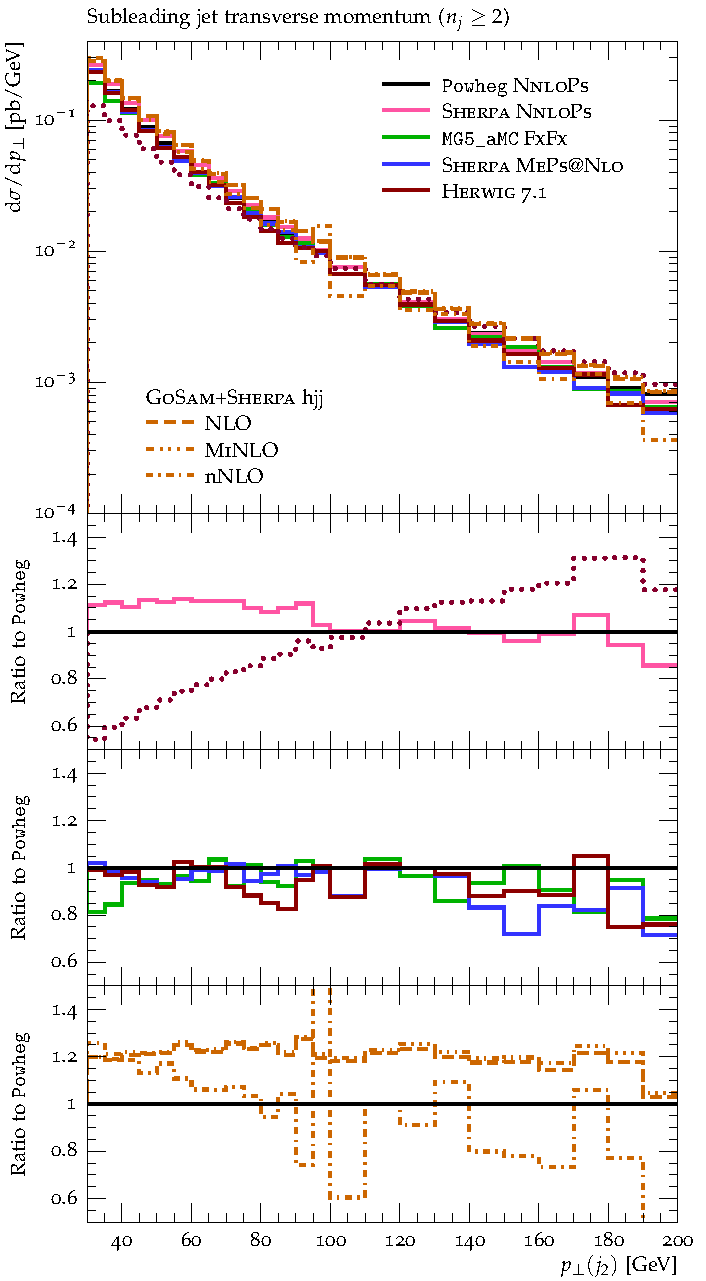
\includegraphics[width=0.47\textwidth]{figures/hjetscomp_u_jet2_pT_incl.pdf}
  \hfill
  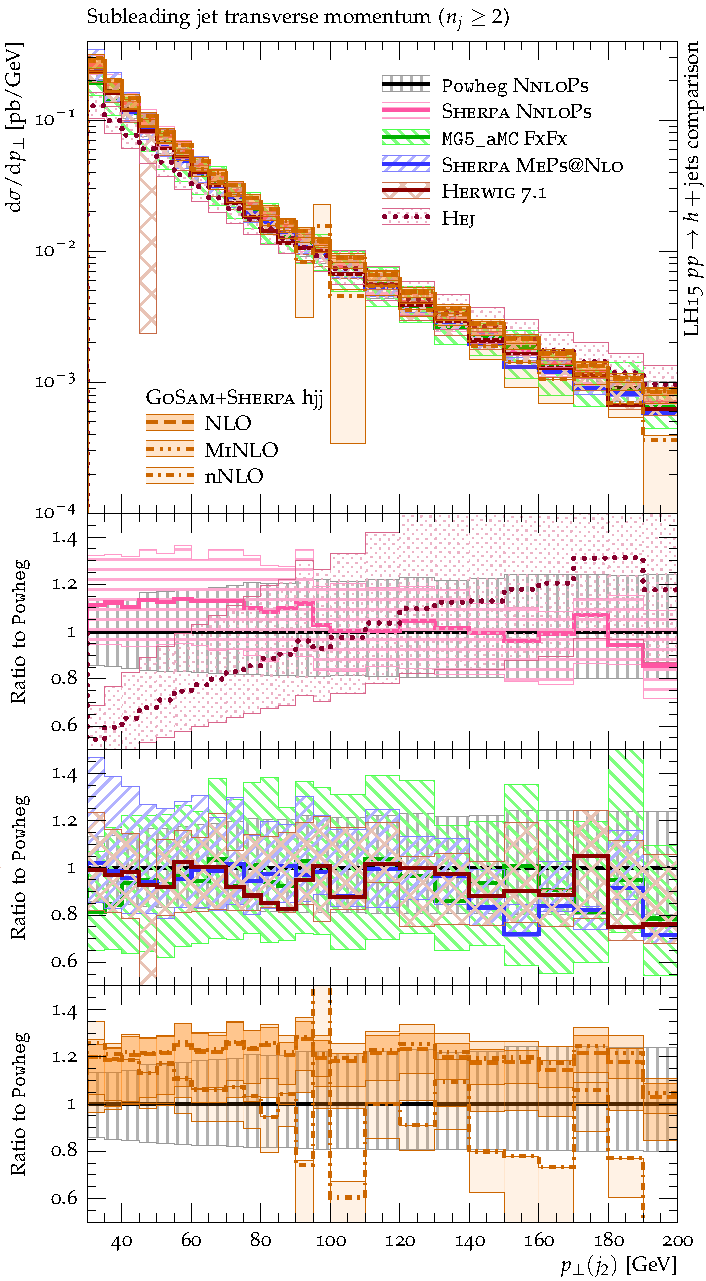
\includegraphics[width=0.47\textwidth]{figures/hjetscomp_jet2_pT_incl.pdf}
  \caption{
    The sub-leading jet $p_T$ for $H+\ge2$ jets production without
    (left) and with (right) uncertainties.
    \label{fig:higgscomp:results:2obs:jet2_pt}
  }
\end{figure}

\begin{figure}[t!]
  \centering
  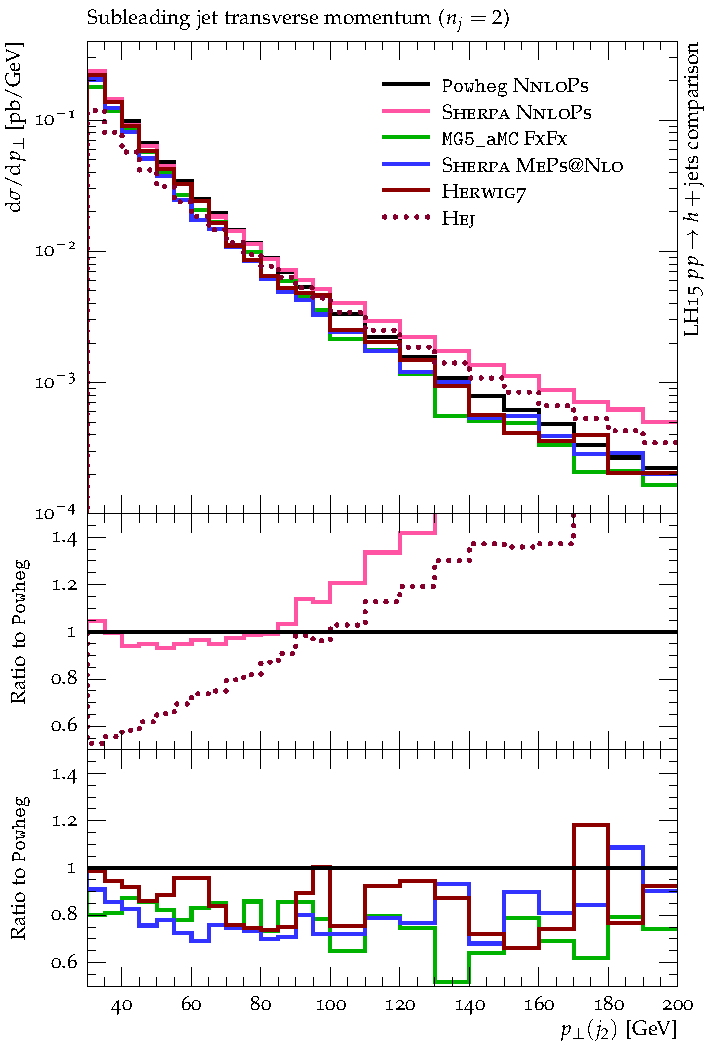
\includegraphics[width=0.47\textwidth]{figures/hjetscomp_u_jet2_pT_excl.pdf}
  \hfill
  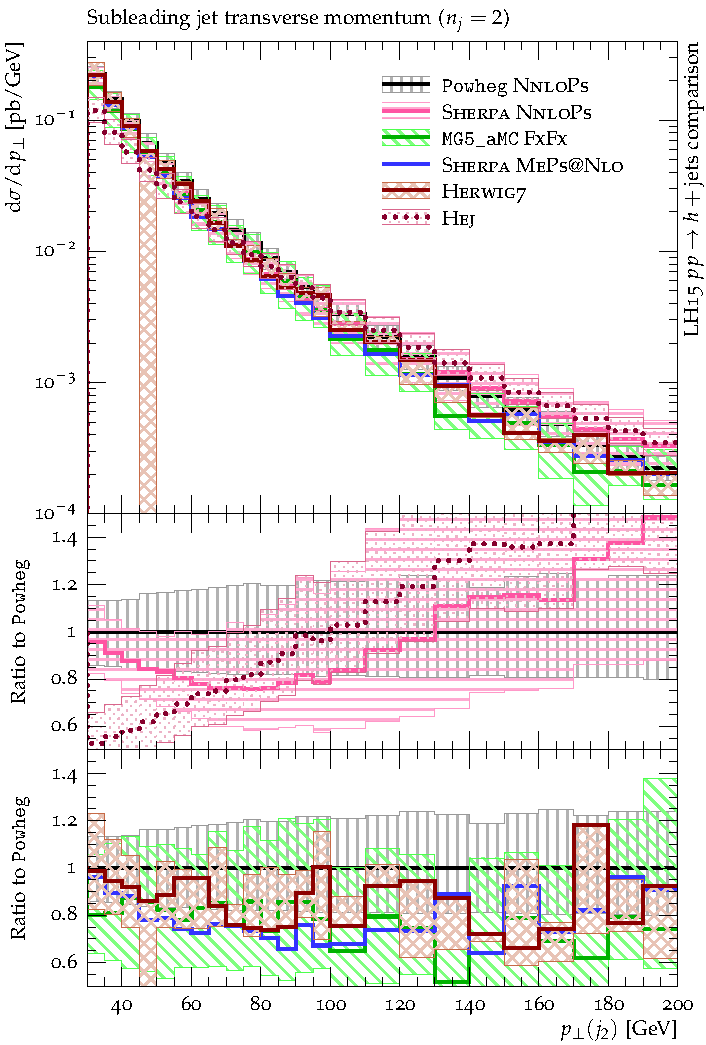
\includegraphics[width=0.47\textwidth]{figures/hjetscomp_jet2_pT_excl.pdf}
  \caption{
    The sub-leading jet $p_T$ for $H$ + exactly 2 jets production without
    (left) and with (right) uncertainties.
    \label{fig:higgscomp:results:2obs:jet2_pt}
  }
\end{figure}

The sub-leading jet $p_T$ for $H+\ge2$ jets is shown in the upper row
of Figure~\ref{fig:higgscomp:results:2obs:jet2_pt}.  The agreement
among the ME+PS predictions and between the ME+PS and fixed order
predictions of gosam is better than in the case of the leading
jets. With two or more jets in the final state, meaningful predictions
to HEJ can be made for the first time.

The sub-leading jet $p_T$ for $H$ + exactly 2 jets is shown in the
lower panel of Figure~\ref{fig:higgscomp:results:2obs:jet2_pt}.
Here, MG5, Sherpa and Herwig7 lie in reasonable agreement with each
other, but systematically lower than Powheg.

\Todo{physics?}

\begin{figure}[t!]
  \centering
  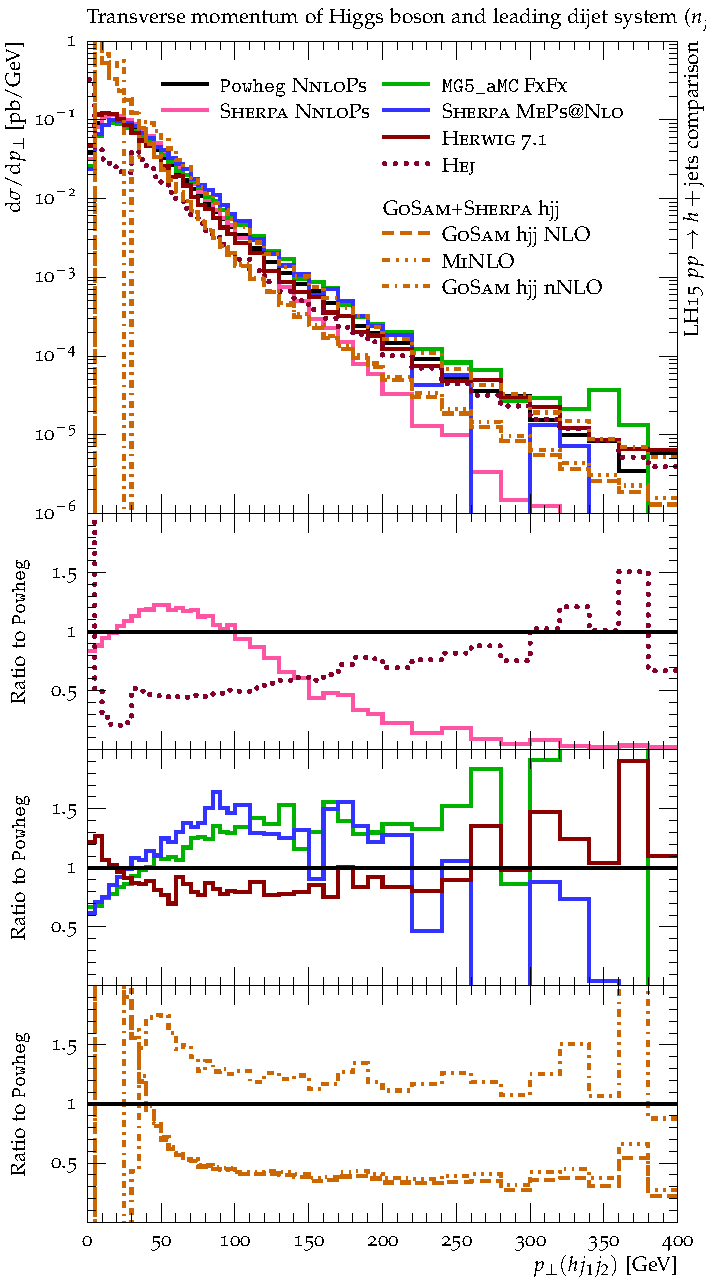
\includegraphics[width=0.47\textwidth]{figures/hjetscomp_u_Hjj_pT_incl.pdf}
  \hfill
  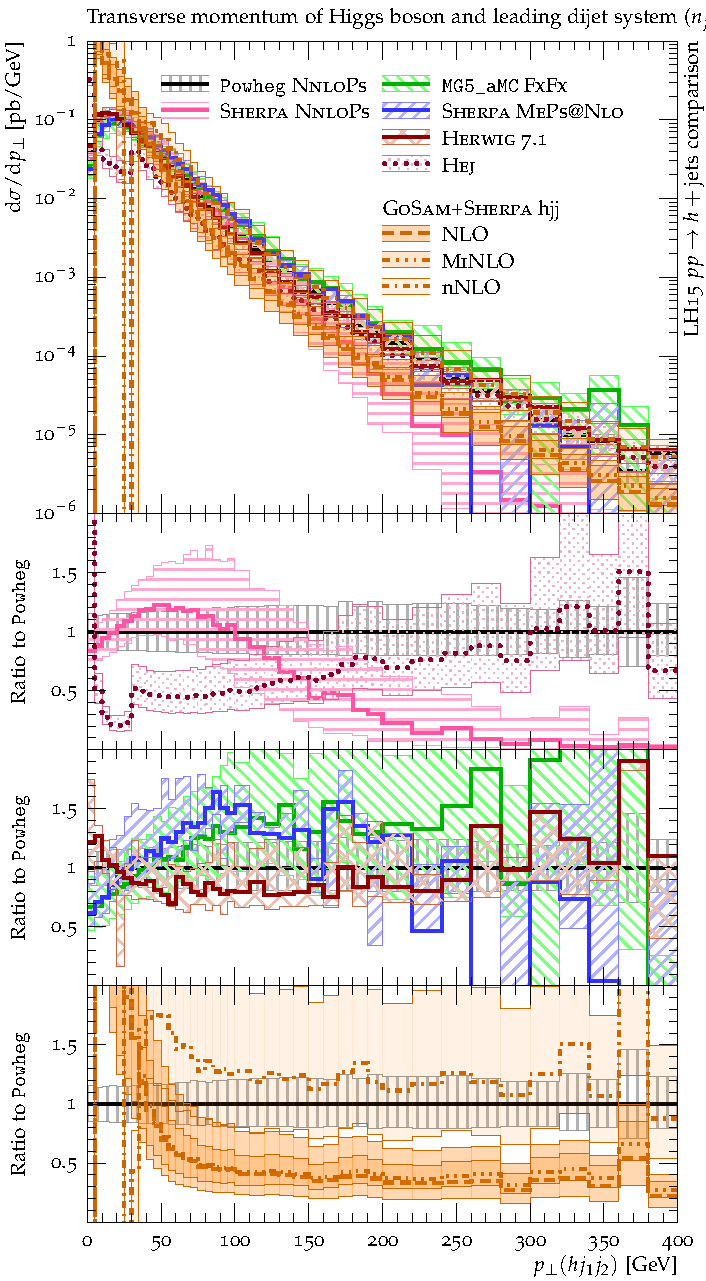
\includegraphics[width=0.47\textwidth]{figures/hjetscomp_Hjj_pT_incl.pdf}
  \caption{
    The transverse momentum of the Higgs boson plus two leading jet
    system without (left) and with (right) uncertainties.
    \label{fig:higgscomp:results:2obs:hjj_pt}
  }
\end{figure}

The transverse momentum of the Higgs boson plus two leading jet system
is shown in Figure~\ref{fig:higgscomp:results:2obs:hjj_pt}. Varying
behavior is also observed here, with MG5 and Sherpa being having a
slope with respect to Powheg at low $p_T$ and being somewhat higher at
high $p_T$, while Herwig7 is again somewhat lower than Powheg at high
$p_T$. The gosam $H+\ge2$ jet prediction is much higher than Powheg at
low $p_T$, and significantly lower at high $p_T$.

\Todo{physics!; why does gosam have the behavior it does?}

\begin{figure}[t!]
  \centering
  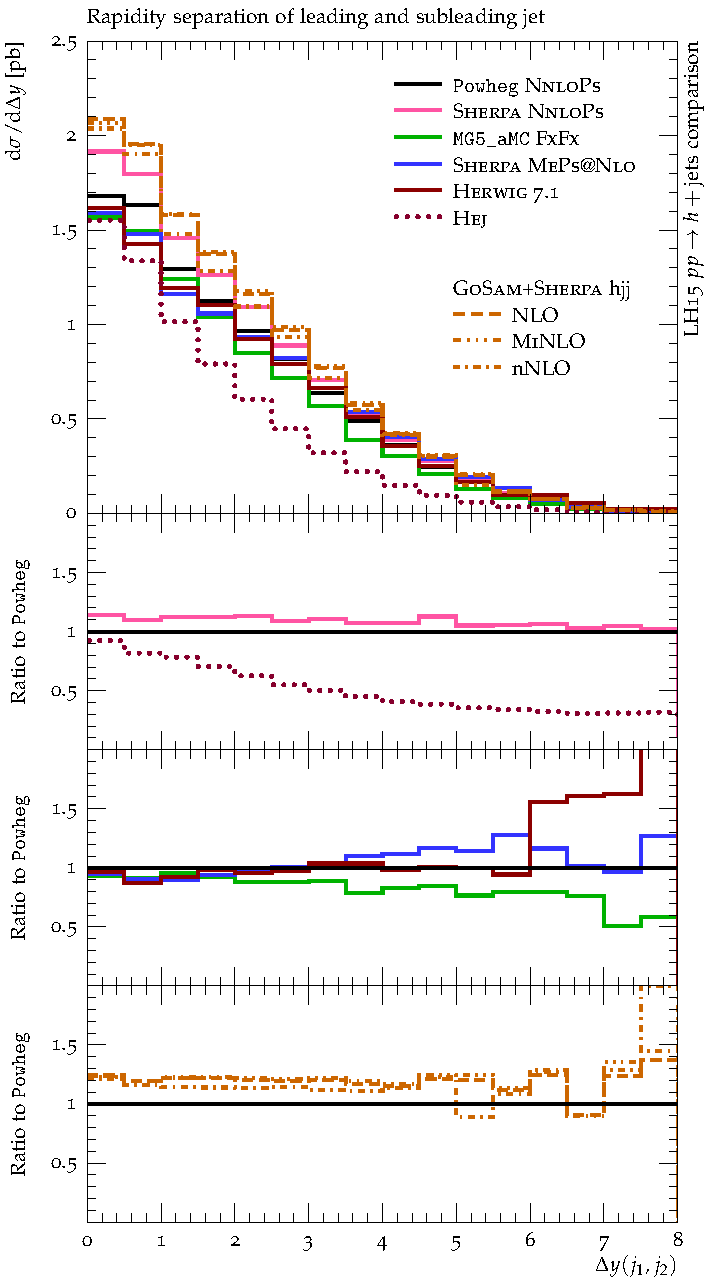
\includegraphics[width=0.47\textwidth]{figures/hjetscomp_u_deltay_jj.pdf}
  \hfill
  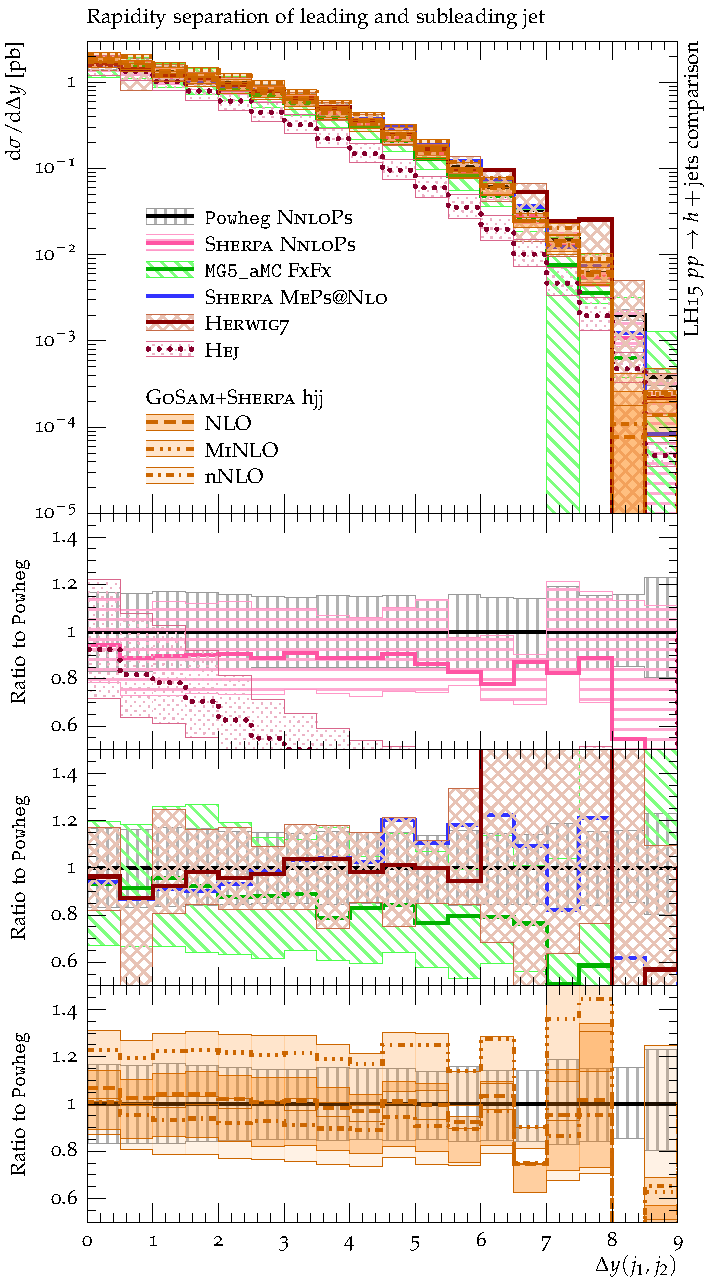
\includegraphics[width=0.47\textwidth]{figures/hjetscomp_deltay_jj.pdf}
  \caption{
    The rapidity separation between the leading and sub-leading jets
    for $H+\ge2$ jets, without (left) and with (right) uncertainties.
    \label{fig:higgscomp:results:2obs:dyjj}
  }
\end{figure}

\begin{figure}[t!]
  \centering
  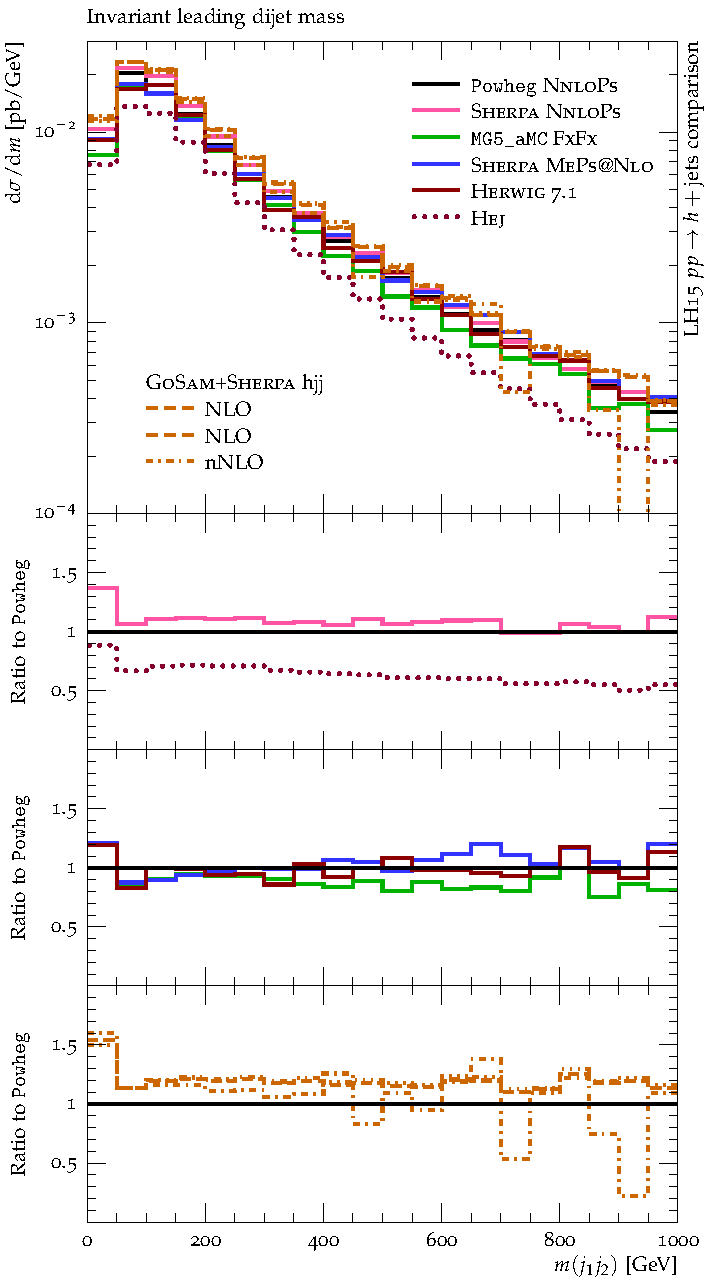
\includegraphics[width=0.47\textwidth]{figures/hjetscomp_u_dijet_mass.pdf}
  \hfill
  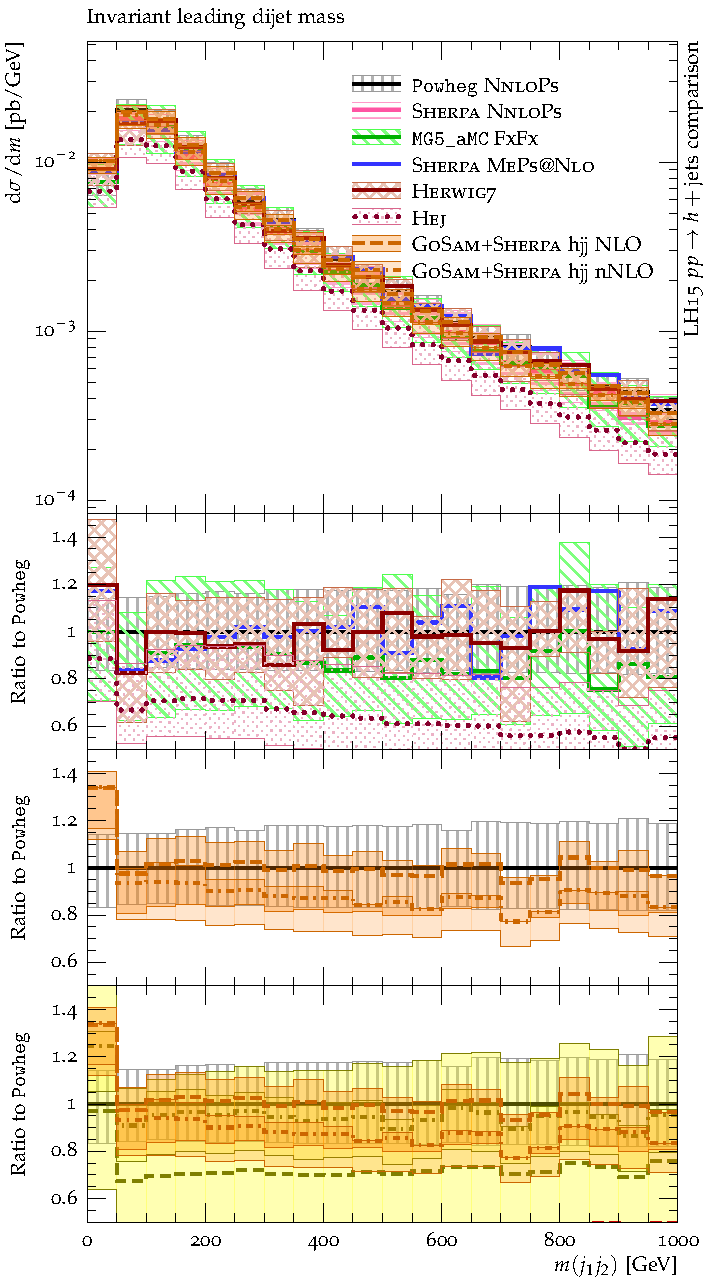
\includegraphics[width=0.47\textwidth]{figures/hjetscomp_dijet_mass.pdf}
  \caption{
    The invariant mass of the leading dijet system without (left) and
    with (right) uncertainties.
    \label{fig:higgscomp:results:2obs:mjj}
  }
\end{figure}

The rapidity separation between the leading and sub-leading jets is
shown in Figure~\ref{fig:higgscomp:results:2obs:dyjj}, for $H+\ge2$
jets. MG5 is lower than Powheg at high $\Delta y$ (while Sherpa is
slightly higher).  Powheg is in good agreement with the fixed order
gosam results for $H+\ge2$ jets. Similar conclusions hold for for the
dijet mass distribution, as shown in
Figure~\ref{fig:higgscomp:results:2obs:mjj}, although the differences
among predictions are smaller.

\begin{figure}[t!]
  \centering
  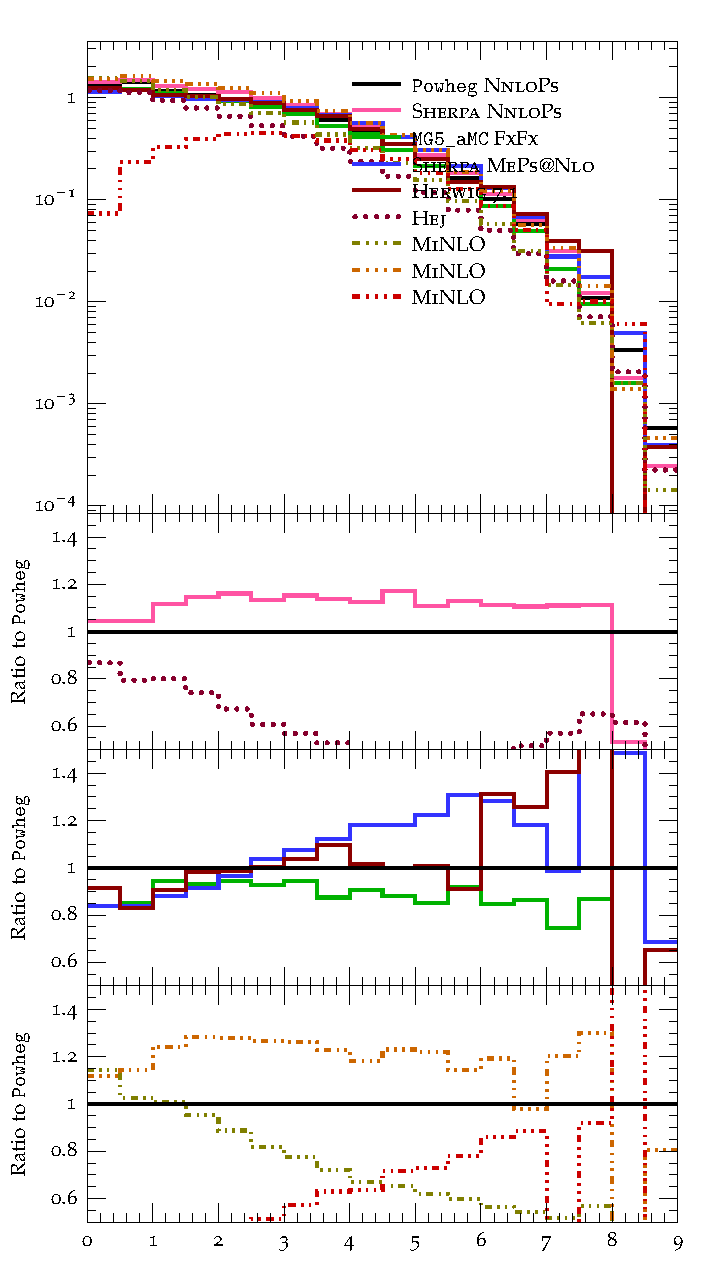
\includegraphics[width=0.47\textwidth]{figures/hjetscomp_u_jjfb_dy.pdf}
  \hfill
  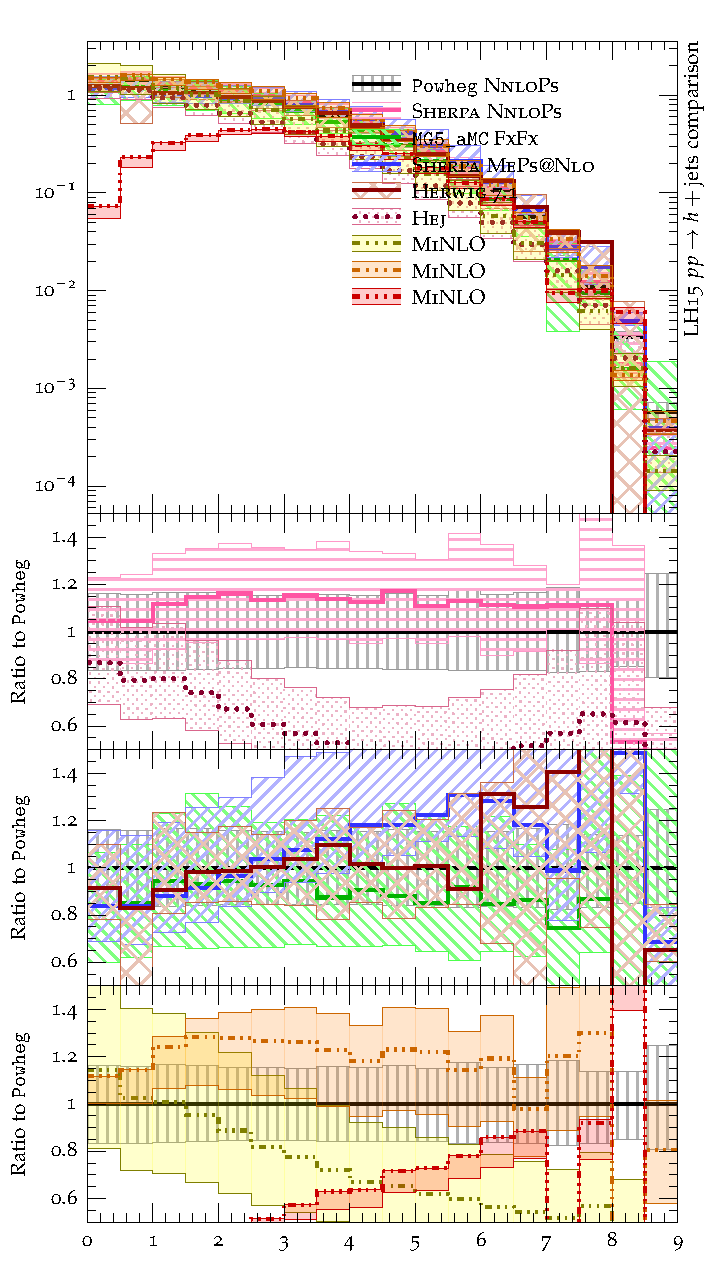
\includegraphics[width=0.47\textwidth]{figures/hjetscomp_jjfb_dy.pdf}
  \caption{
    The rapidity separation between the two most forward-backward jets
    for $H+\ge2$ jets, without (left) and with (right) uncertainties. 
    \label{fig:higgscomp:results:2obs:dyjj_fb}
  }
\end{figure}

The rapidity separation between the two most forward-backward jets is
shown in Figure~\ref{fig:higgscomp:results:2obs:dyjj_fb}. As for the
$p_T$-ordered distribution, MG5 is lower than Powheg at high $\Delta
y$ while Sherpa is higher. Powheg now has a slope compared to the
Gosam NLO results, but, interestingly, not compared to the nNLO
results.

\begin{figure}[t!]
  \centering
  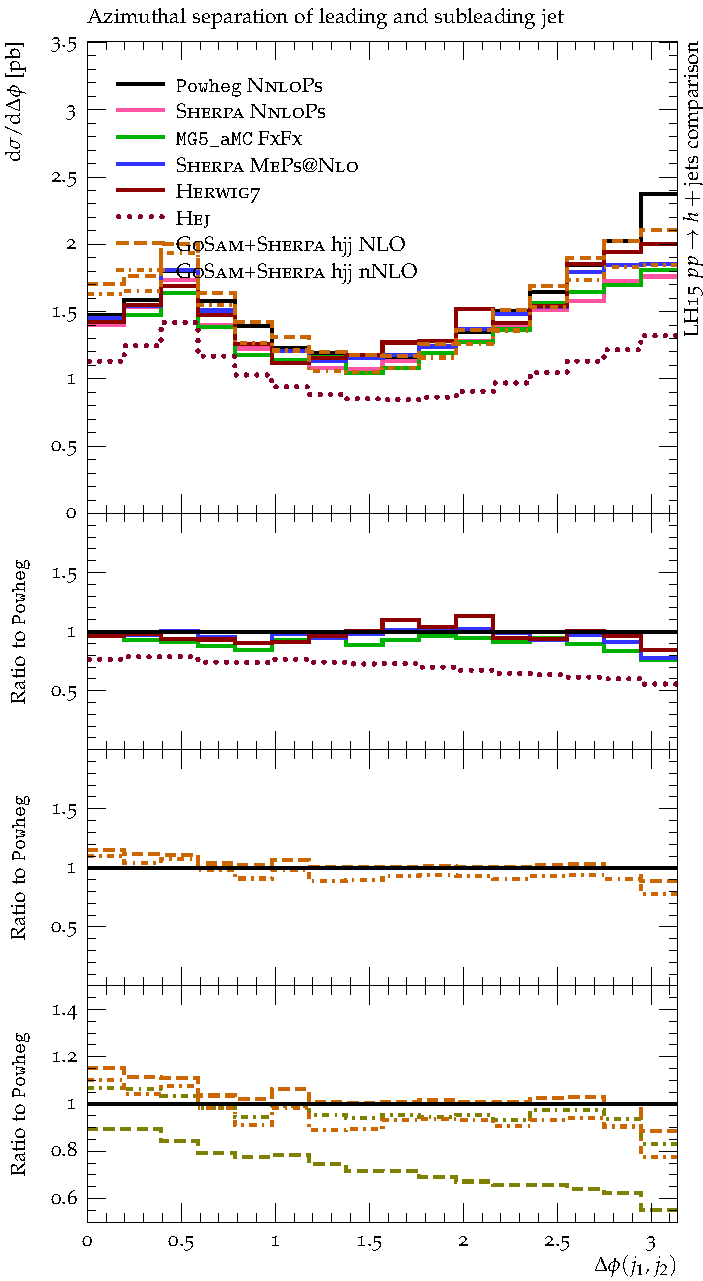
\includegraphics[width=0.47\textwidth]{figures/hjetscomp_u_deltaphi_jj_incl.pdf}
  \hfill
  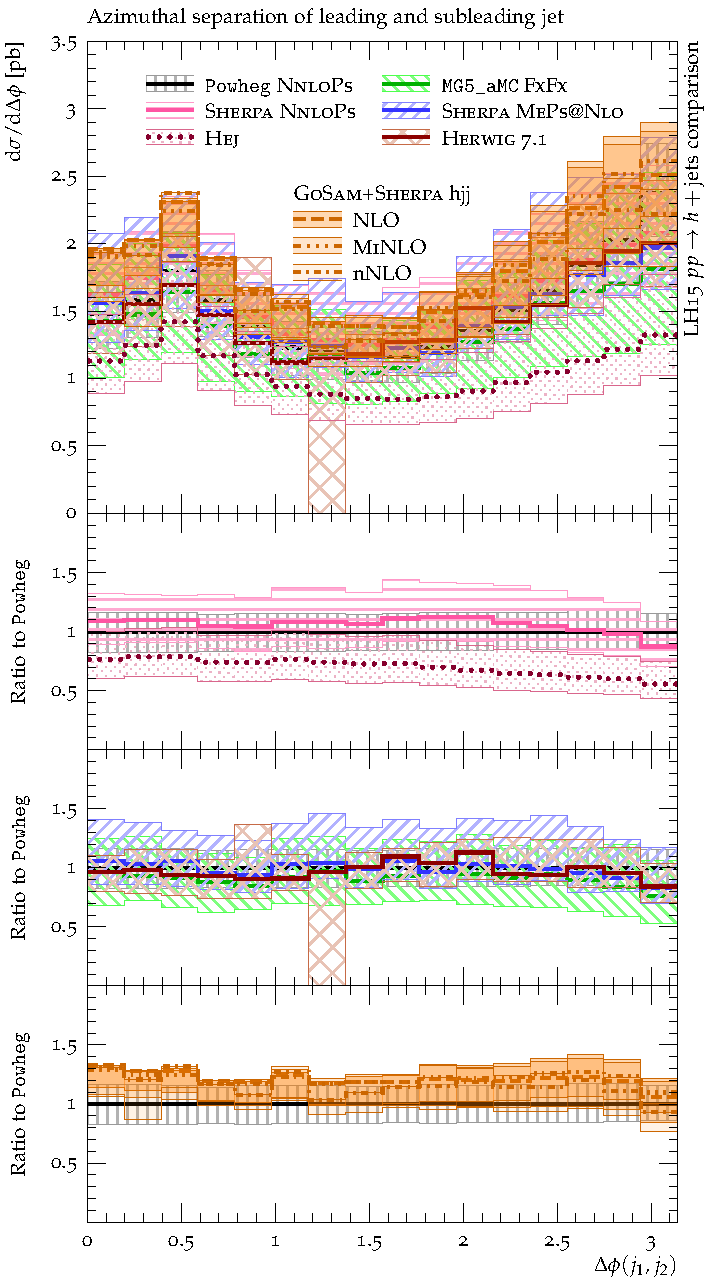
\includegraphics[width=0.47\textwidth]{figures/hjetscomp_deltaphi_jj_incl.pdf}
  \caption{
    The $\Delta\phi$ separation between the two leading jets for
    $H+\ge2$ jets, without (left) and with (right) uncertainties. 
    \label{fig:higgscomp:results:2obs:dphi_jj}
  }
\end{figure}

The $\Delta\phi$ separation between the two leading jets is shown in
Figure~\ref{fig:higgscomp:results:2obs:dphi_jj}. All predictions are
in good agreement with each other, except for HEJ, which has a leading
order normalization. Similar distributions (and agreement) are
observed if the two most forward-backward jets are chosen instead.



\clearpage
\subsection{VBF observables}
\label{sec:hjetscomp:results:VBFobs}

To single out observables with VBF kinematics, additional cuts are
placed, requiring the dijet mass distribution formed from the leading
and sub-leading jets to have a mass greater than 400 GeV, and in
addition requiring the two leading jets to have a rapidity separation
greater than 2.8 (VBF cuts). An alternative set of cuts requires that
any two jets satisfy the preceding criteria (VBF2 cuts).

\begin{figure}[t!]
  \centering
  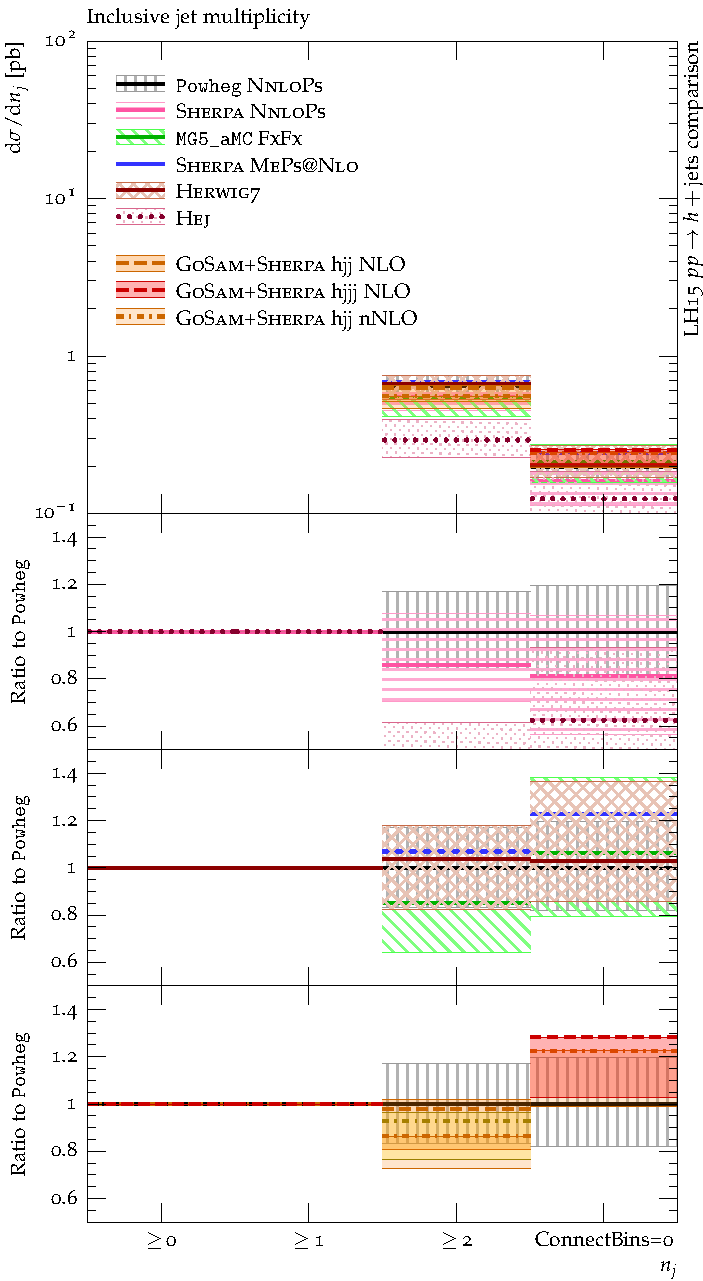
\includegraphics[width=0.47\textwidth]{figures/hjetscomp_NJet_incl_30_VBF.pdf}
  \hfill
  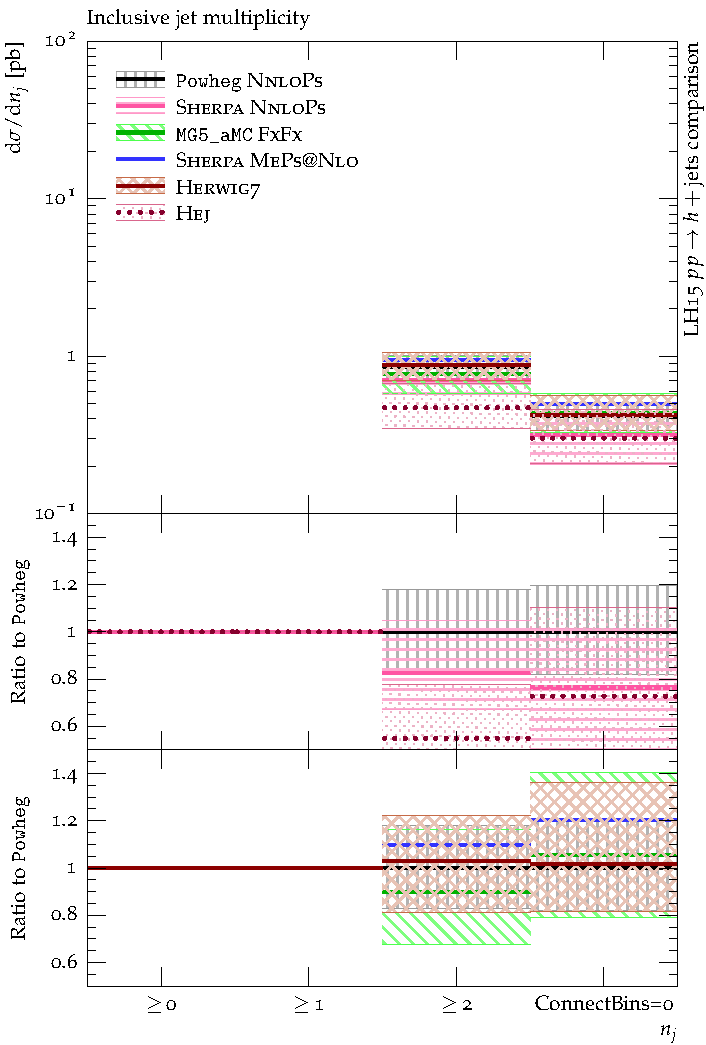
\includegraphics[width=0.47\textwidth]{figures/hjetscomp_NJet_incl_30_VBF2.pdf}
  \caption{\label{fig:higgscomp:results:inclobs:njets_VBF}
    The inclusive jet multiplicities with VBF (left) and VBF2 (right)
    cuts.  }
\end{figure}

The inclusive jet multiplicity distributions with VBF cuts are shown
in Figure~\ref{fig:higgscomp:results:inclobs:njets_VBF}. The hierarchy
is essentially the same as for the inclusive jet multiplicity
distribution without any cuts. The differences among the predictions
are somewhat smaller with the VBF2 cuts than with the VBF cuts.

\begin{figure}[t!]
  \centering
  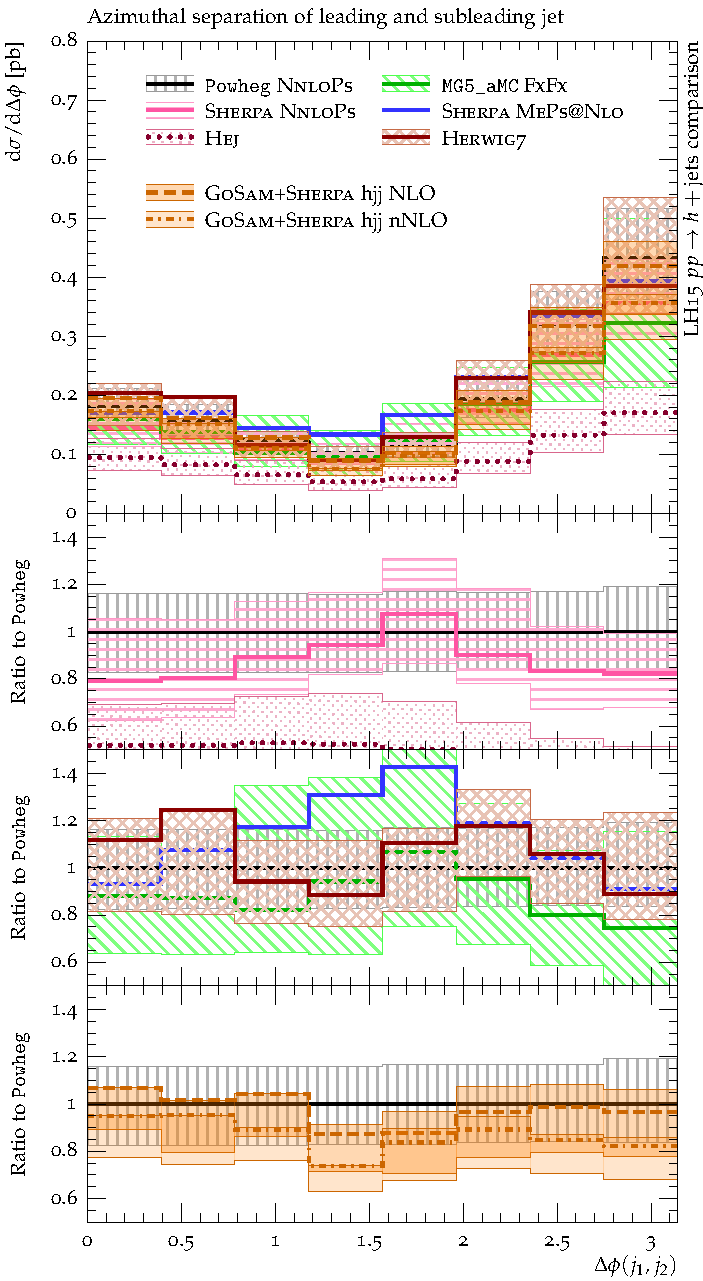
\includegraphics[width=0.47\textwidth]{figures/hjetscomp_deltaphi_jj_VBF.pdf}
  \hfill
  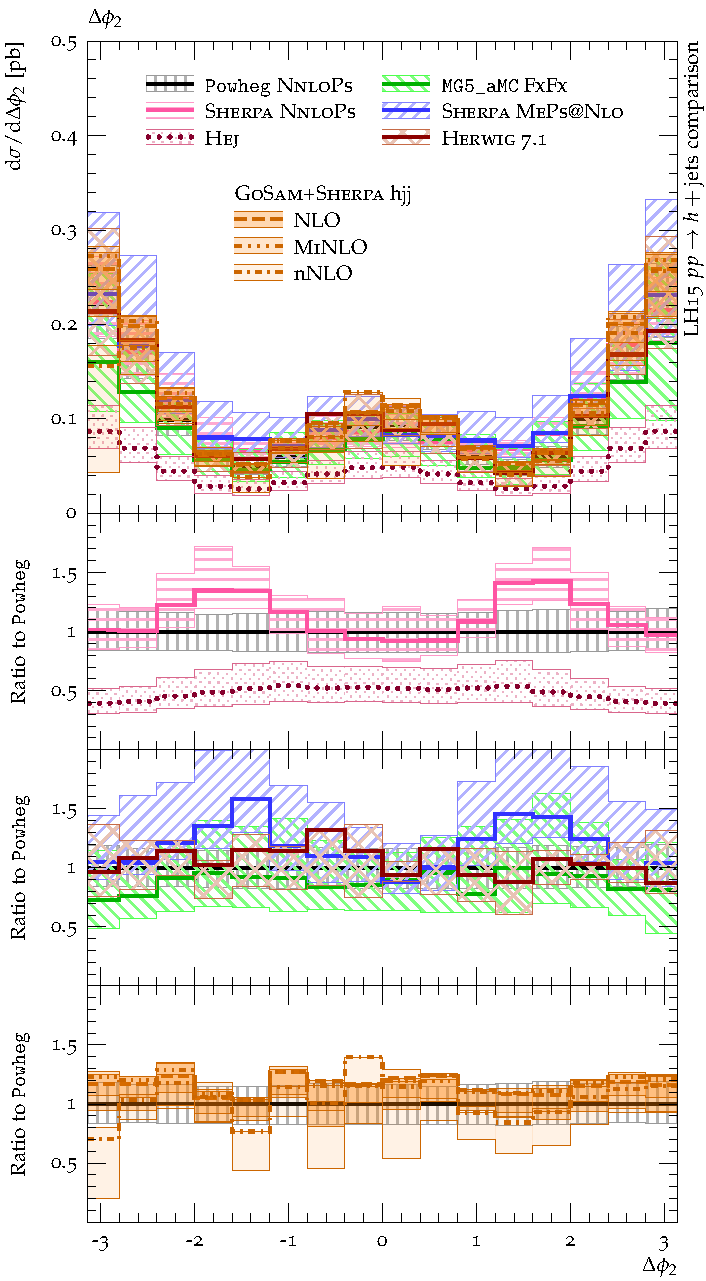
\includegraphics[width=0.47\textwidth]{figures/hjetscomp_deltaphi2_VBF.pdf}
  \caption{
    Azimuthal separation of the leading jet pair (left) and 
    $\Delta\phi_2$ (right) after applying VBF cuts in $H+\ge2$ jet
    production.
    \label{fig:higgscomp:results:VBFobs:dphijj_phi2}
    \Todo{Joey suggests to add no-uncertainty plot versions here too.}
  }
\end{figure}

The $\Delta\phi$ separation between the two leading jets applying the
VBF cuts is shown in
Figure~\ref{fig:higgscomp:results:VBFobs:dphijj_phi2}. All predictions
are in reasonable agreement with each other, although not as good
agreement as for the inclusive case. Similar distributions (and
agreement) are observed if the two most forward-backward jets are
chosen instead.

\Todo{I'm not sure what other observables to put into this section. It
  would have been nice to have the 3rd jet pT distribution with VBF
  cuts.}



\clearpage
\subsection{Multijet observables}
\label{sec:hjetscomp:results:mjobs}

\begin{figure}[t!]
  \centering
  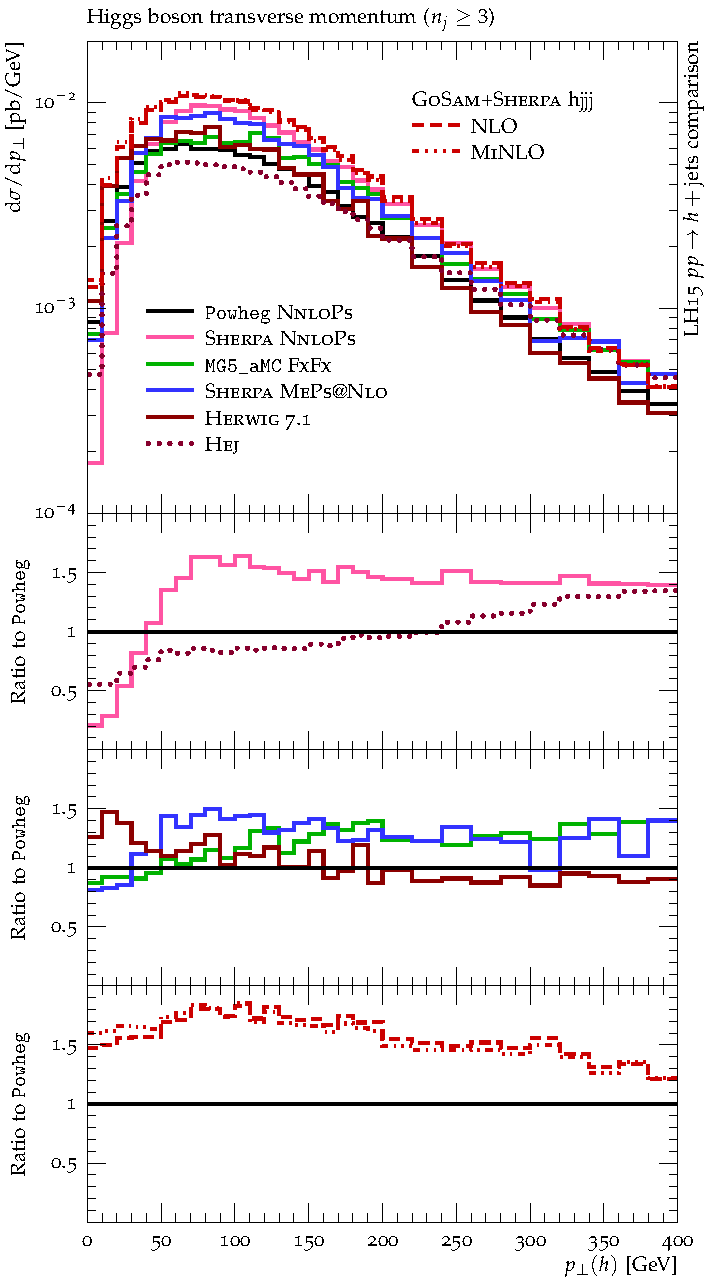
\includegraphics[width=0.47\textwidth]{figures/hjetscomp_u_H_jjj_pT_incl.pdf}
  \hfill
  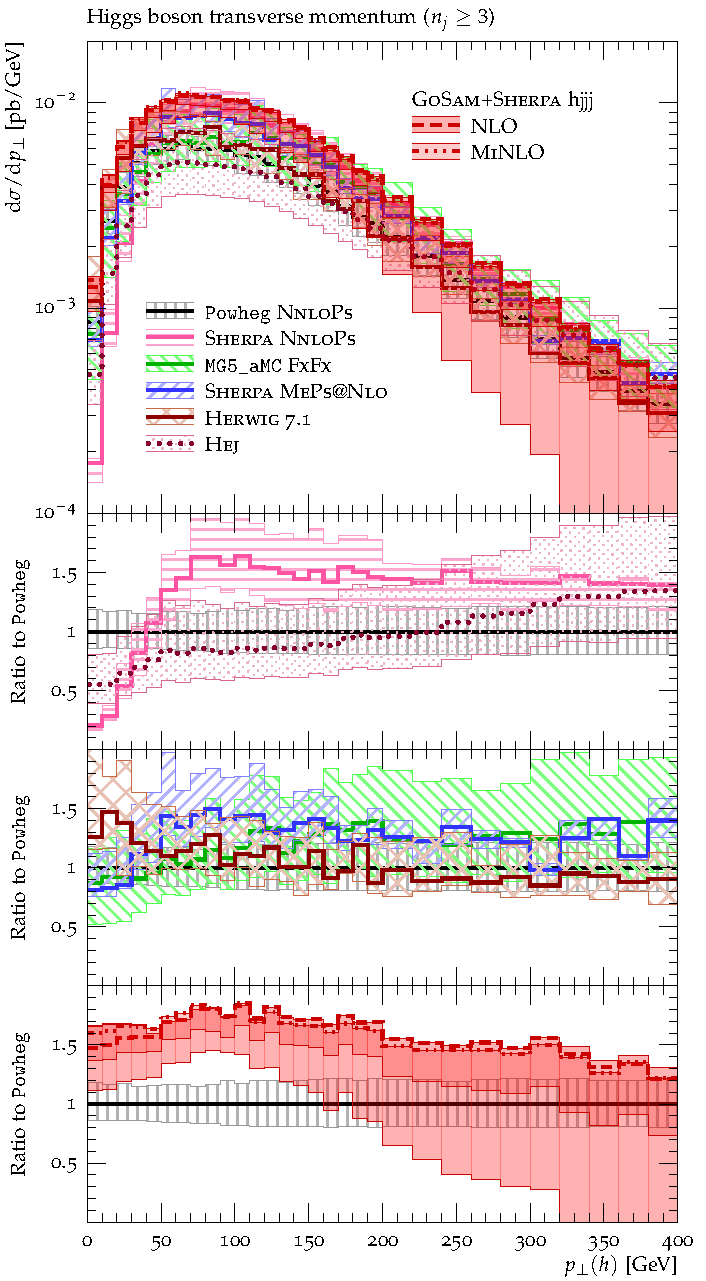
\includegraphics[width=0.47\textwidth]{figures/hjetscomp_H_jjj_pT_incl.pdf}
  \caption{
    The Higgs boson transverse momentum in the presence of at least three 
    jets, shown without (left) and with (right) theoretical uncertainties.
    \label{fig:higgscomp:results:mobs:hpt_j3}
  }
\end{figure}

The Higgs boson transverse momentum distribution for $H+\ge3$ jets is
shown in Figure~\ref{fig:higgscomp:results:mobs:hpt_j3}. MG5 and
Sherpa tend to be higher than Powheg (where the jet is produced by a
parton shower), and similar to that from Gosam $H+\ge3$ jets, which
has the correct NLO $K$-factor.

\begin{figure}[t!]
  \centering
  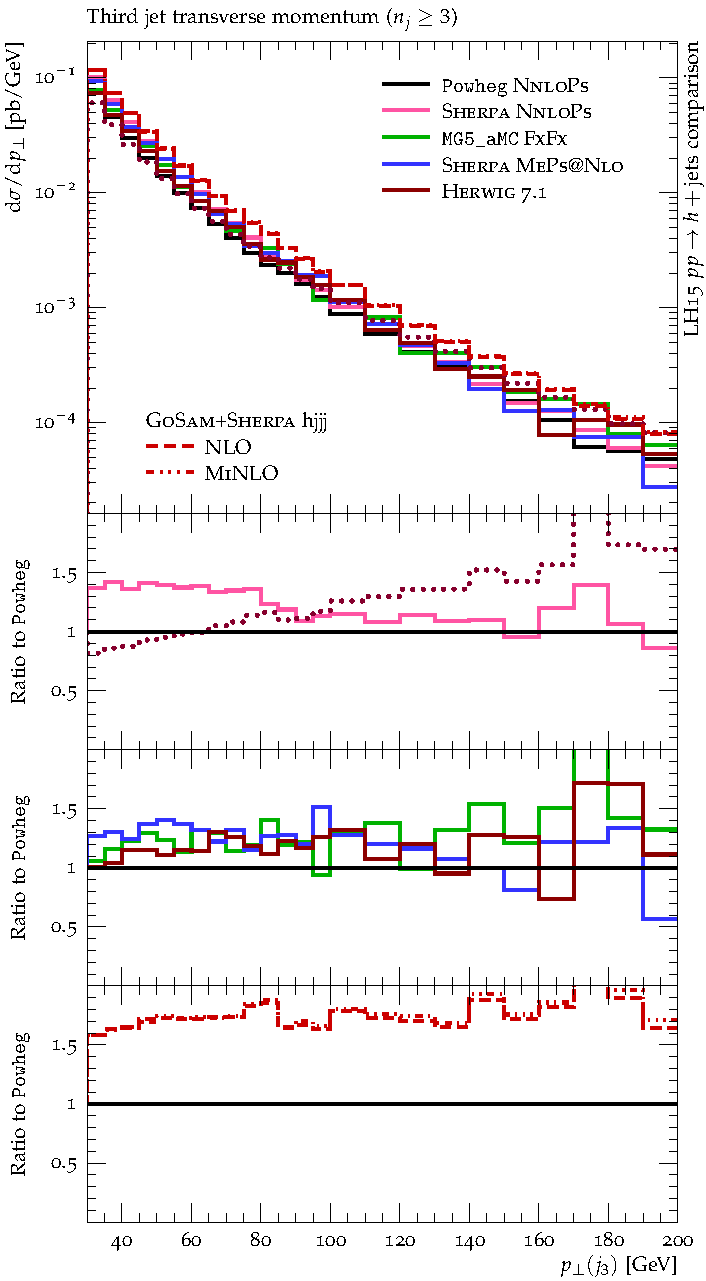
\includegraphics[width=0.47\textwidth]{figures/hjetscomp_u_jet3_pT_incl.pdf}
  \hfill
  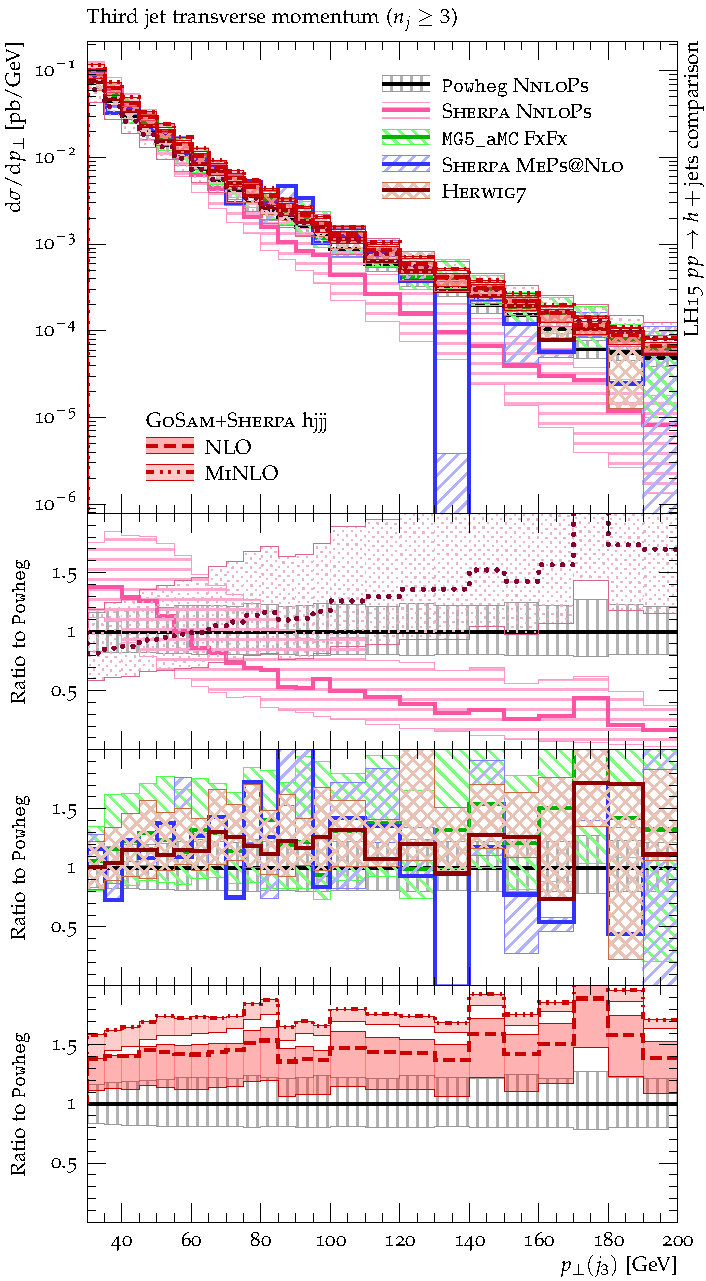
\includegraphics[width=0.47\textwidth]{figures/hjetscomp_jet3_pT_incl.pdf}
  \caption{
    The third jet transverse momentum distribution for $H+\ge3$ jets
    shown without (left) and with (right) theoretical uncertainty bands.
    \label{fig:higgscomp:results:mobs:j3pt}
  }
\end{figure}

The third jet $p_T$ for $H+\ge3$ jets is shown in
Figure~\ref{fig:higgscomp:results:mobs:j3pt}. MG5, Herwig7 and Sherpa
tend to be higher than Powheg (where the jet is produced by a parton
shower), but lower than that from Gosam $H+\ge3$ jets, which has the
correct NLO $K$-factor. The multijet phase space results in smaller
Sudakov effects, and thus better agreement with the fixed-order
predictions.

\begin{figure}[t!]
  \centering
  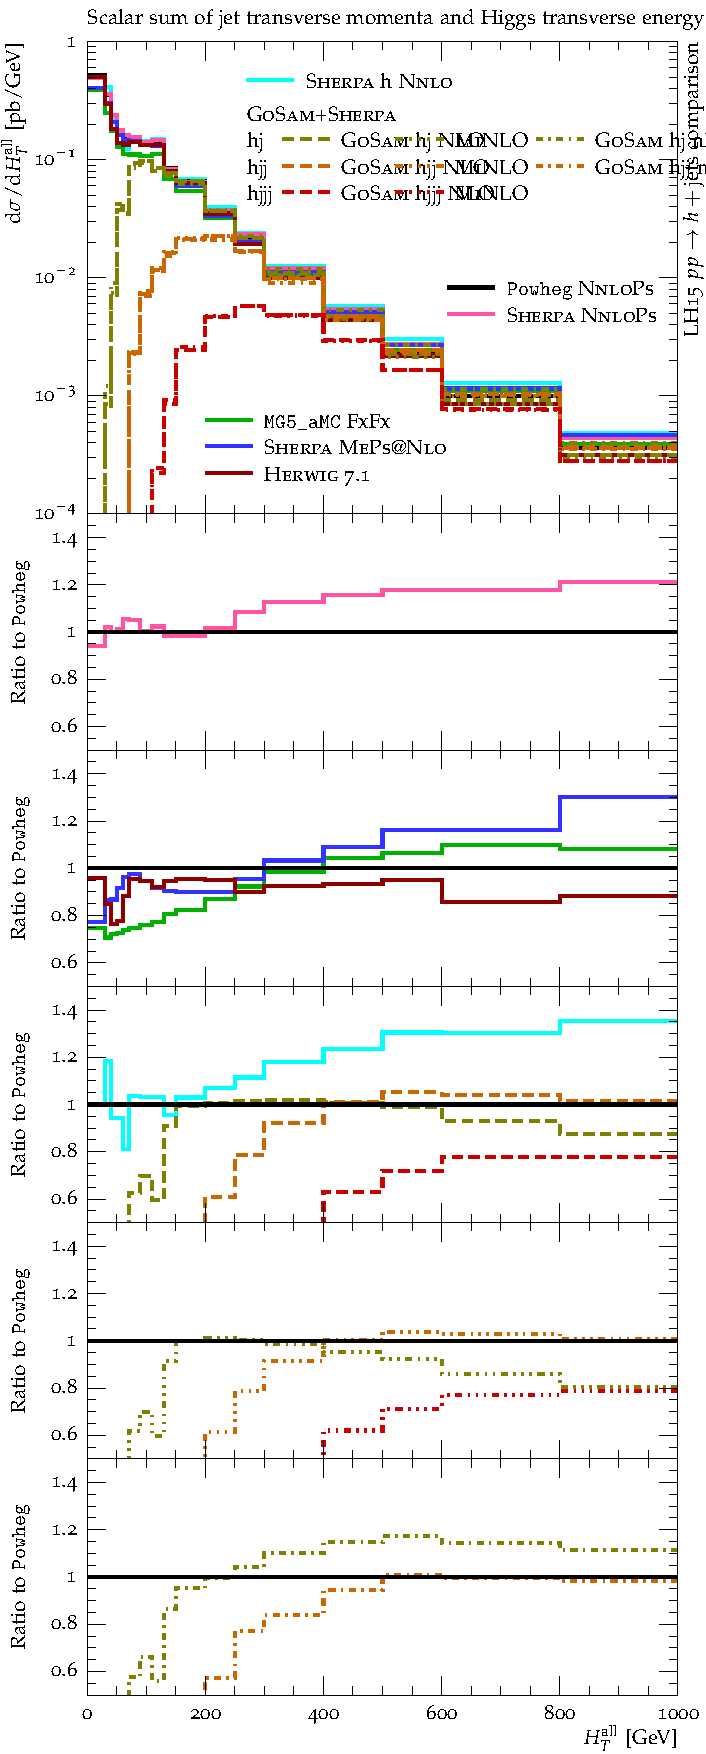
\includegraphics[width=0.47\textwidth]{figures/hjetscomp_u_HT_all.pdf}
  \hfill
  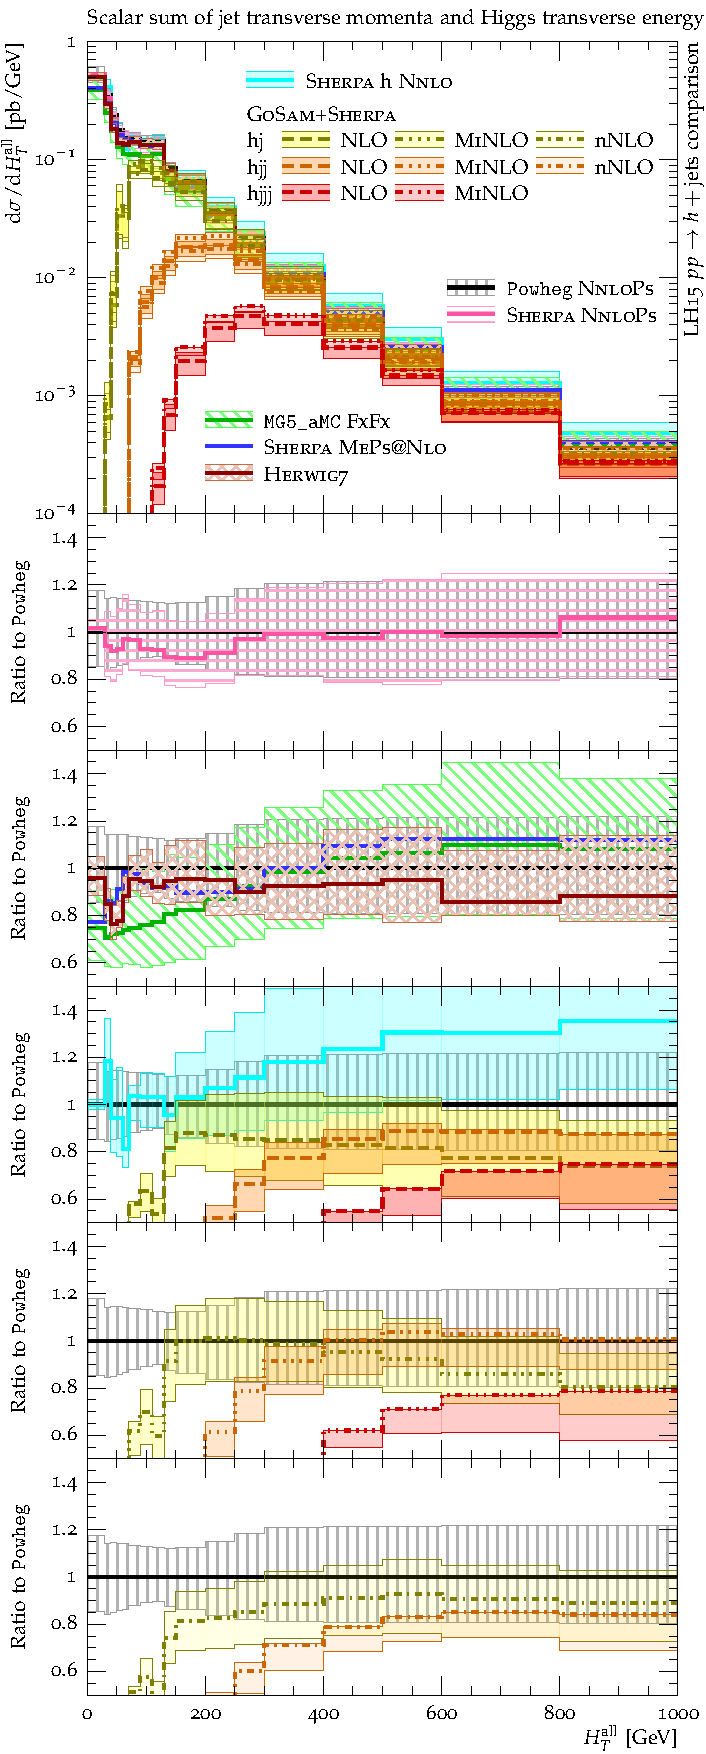
\includegraphics[width=0.47\textwidth]{figures/hjetscomp_HT_all.pdf}
  \caption{
    The $H_T$ distribution for $H+\ge1$ jets \Todo{is this correct?}
    without (left) and with (right) uncertainties.
    \label{fig:higgscomp:results:mobs:HT_all}
  }
\end{figure}

\begin{figure}[t!]
  \centering
  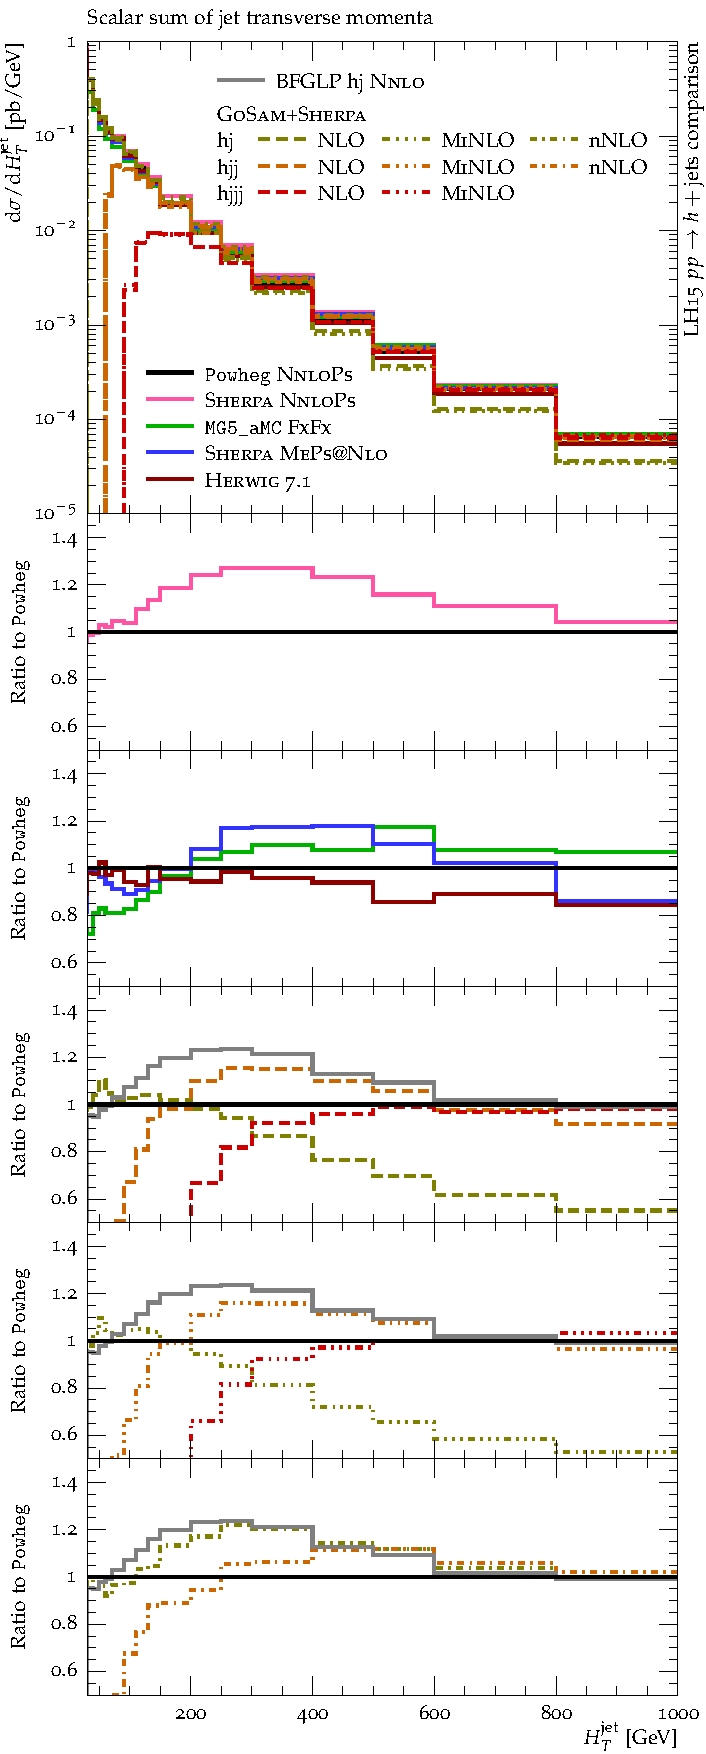
\includegraphics[width=0.47\textwidth]{figures/hjetscomp_u_HT_jets.pdf}
  \hfill
  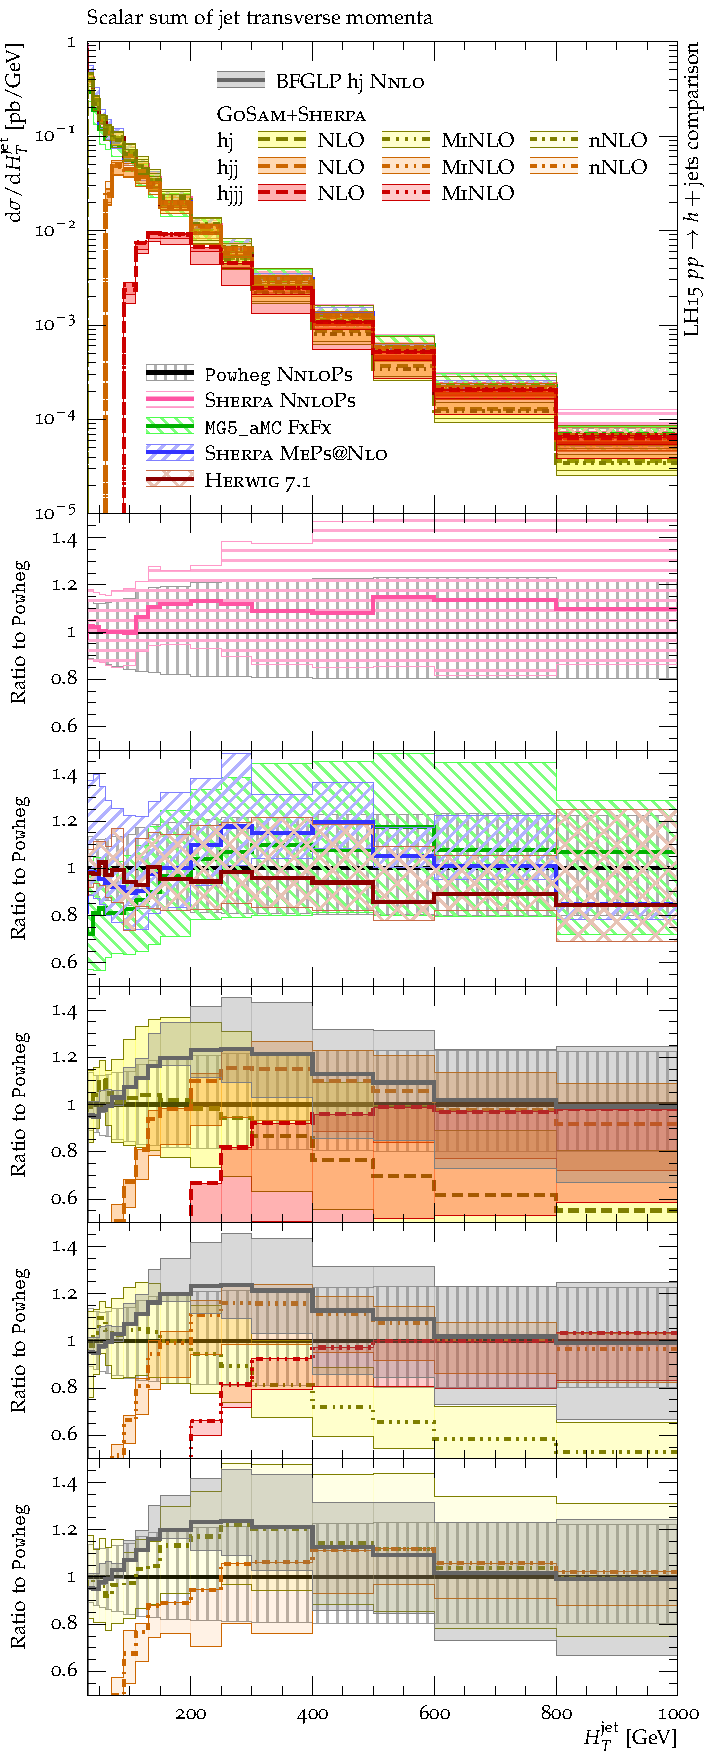
\includegraphics[width=0.47\textwidth]{figures/hjetscomp_HT_jets.pdf}
  \caption{
    The $H_{T,\mathrm{jets}}$ distribution for $H+\ge1$ jet final
    states, without (left) and with (right) uncertainties.
    \label{fig:higgscomp:results:mobs:HT_jets}
  }
\end{figure}

The $H_T$ distribution (sum of the transverse momenta for all objects
in the final state) for $H+\ge1$ jets is shown in
Figure~\ref{fig:higgscomp:results:mobs:HT_all} and the $H_T$
distribution for jets only is shown in in
Figure~\ref{fig:higgscomp:results:mobs:HT_jets}. \Todo{Jan: we don't
  consider $H$ decays, so the all-objects HT would be different from
  an experimental point of view. Do we want both HTs and clarify or
  only the HTjets.}
MG5 and Sherpa tend to be lower than Powheg at low $H_T$ and higher at
large $H_T$. The fixed order predictions (from gosam and from $H+\ge1$
jet at NNLO) are consistently lower than Powheg (although the NNLO
prediction does agree with Powheg in the 150-300 GeV range for
$HT_{jets}$).



\clearpage
\subsection{Jet veto observables}
\label{sec:hjetscomp:results:jvobs}

\begin{figure}[t!]
  \centering
  \includegraphics[width=0.47\textwidth]{figures/hjetscomp_u_xs_jet_veto_j0.pdf}
  \hfill
  \includegraphics[width=0.47\textwidth]{figures/hjetscomp_xs_jet_veto_j0.pdf}
  \caption{
    The exclusive zero jet cross section in dependence on / as a
    function of the vetoed minimal leading jet transverse momentum,
    without (left) and with (right) uncertainties.
    \label{fig:higgscomp:results:jvobs:jvxs0}
  }
\end{figure}

The cross section for the production of a Higgs boson and no
additional jets as a function of the minimum jet transverse momentum
is shown in Figure~\ref{fig:higgscomp:results:jvobs:jvxs0}. Good
agreement with the Powheg predictions is observed above a jet veto cut
of approximately 20~GeV.

\begin{figure}[t!]
  \centering
  \includegraphics[width=0.47\textwidth]{figures/hjetscomp_u_xs_jet_veto_j1_30.pdf}
  \hfill
  \includegraphics[width=0.47\textwidth]{figures/hjetscomp_xs_jet_veto_j1_30.pdf}
  \caption{
    The cross
    section for a Higgs boson plus exactly one jet as a function on
    the vetoed minimal second jet transverse momentum without
    (left) and with (right) uncertainties. Also, Joey picked the
    30~GeV requirement for $H$ or jet1.
    \label{fig:higgscomp:results:jvobs:jvxs1j}
  }
\end{figure}

\begin{figure}[t!]
  \centering
  %\includegraphics[width=0.47\textwidth]{Micon.pdf}
  \includegraphics[width=0.47\textwidth]{figures/hjetscomp_u_xs_jet_veto_j1_200.pdf}
  \hfill
  \includegraphics[width=0.47\textwidth]{figures/hjetscomp_xs_jet_veto_j1_200.pdf}
  \caption{
    The cross
    section for a Higgs boson plus exactly one jet as a function on
    the vetoed minimal second jet transverse momentum without
    (left) and with (right) uncertainties. Also, Joey picked the
    30~GeV requirement for $H$ or jet1.
    \label{fig:higgscomp:results:jvobs:jvxs1j}
  }
\end{figure}

The cross section for the production of $H$ plus exactly one jet and
no additional jets as a function of the sub-leading minimum jet
transverse momentum is shown in
Figure~\ref{fig:higgscomp:results:jvobs:jvxs1h_jvxs1j}. Again, good
agreement with the Powheg predictions (almost perfect for Herwig7 and
Sherpa) is observed above a jet veto cut of approximately 20~GeV. The
effects of the higher central scale for MG5 is evident.

\begin{figure}[t!]
  \centering
  \includegraphics[width=0.47\textwidth]{figures/hjetscomp_u_xs_central_jet_veto_VBF.pdf}
  \hfill
  \includegraphics[width=0.47\textwidth]{figures/hjetscomp_xs_central_jet_veto_VBF.pdf}
  \caption{
    The cross section after VBF cuts as a function of the rapidity
    distance of the two ($p_T$-ordered) tagging jets. A veto has been
    applied on the leading central jet with transverse momentum larger
    than 30~GeV.
    \label{fig:higgscomp:results:jvobs:cjvxsvbf}
  }
\end{figure}

The central jet veto cross section for $H+\ge2$ jets is shown as a
function of the rapidity separation for the two leading jets in
Figure~\ref{fig:higgscomp:results:jvobs:cjvxsvbf}. MG5, Sherpa and
Herwig7 are all in excellent agreement with Powheg.
